\documentclass[11pt]{article}
\usepackage[utf8]{inputenc}
\usepackage[T1]{fontenc}
\usepackage{textcomp}
\usepackage[a4paper,margin=2.1cm]{geometry}
\usepackage{amsmath,amssymb}
\usepackage{graphicx}
\usepackage{tikz}
\usetikzlibrary{positioning,arrows.meta}
\usepackage{xcolor}
\usepackage{mdframed}
\usepackage[colorlinks=true,linkcolor=blue!60!black]{hyperref}
\setlength{\parindent}{0pt}
\setlength{\parskip}{6pt}

\newcommand{\question}[1]{\par\medskip\noindent\textbf{#1}\par}
\newmdenv[linecolor=green!45!black,linewidth=0.8pt,backgroundcolor=green!4,
  innertopmargin=4pt,innerbottommargin=4pt,skipabove=6pt,skipbelow=6pt]{answerbox}

\title{\textbf{Rationalising the Denominator}\\[0.3em]\large Worked Solutions with TikZ Diagrams}
\author{Wisest Maths --- Year 1 A-Level, Algebra (ref \texttt{a6})}
\date{}

\begin{document}
\maketitle
\noindent This document contains all 59 \emph{Rationalising the Denominator} questions, each with a
fully worked solution and a TikZ diagram. The whole topic rests on one idea: \textbf{multiply by a cleverly
chosen form of~$1$}, so the diagrams reflect that:
\begin{itemize}\setlength{\itemsep}{1pt}
  \item \textbf{$\frac{\sqrt a}{\sqrt a}$ cards} for a single-surd denominator;
  \item \textbf{conjugate cards} for a two-term denominator (the difference of two squares clears the surd);
  \item \textbf{solution-flow} diagrams for simplifying, combining, and solving equations;
  \item a \textbf{rectangle} diagram for the area problem.
\end{itemize}
\tableofcontents
\bigskip
\hrule

\section*{Rationalising the Denominator 01\quad\small\texttt{(a6-001)}}
\addcontentsline{toc}{section}{Rationalising the Denominator 01 (a6-001)}
\textit{Difficulty: Foundation \quad\textbar\quad Marks: 1}

\question{Rationalise the denominator: \( \frac{1}{\sqrt{2}} \)}

\textbf{Worked solution.}

\textit{Multiply the top and bottom of the fraction by \( \sqrt{2} \).}
\[\begin{gathered}
\frac{1}{\sqrt{2}} \times \frac{\sqrt{2}}{\sqrt{2}} = \frac{\sqrt{2}}{2}
\end{gathered}\]
Multiplying by \( \frac{\sqrt{2}}{\sqrt{2}} \) does not change the value of the fraction (it equals 1), but it removes the surd from the denominator.

\begin{answerbox}
\textbf{Final answer:}\quad \(\displaystyle \frac{\sqrt{2}}{2}\)
\end{answerbox}
\textbf{Diagram.}

\begin{center}
\resizebox{\ifdim\width>\linewidth \linewidth\else \width\fi}{!}{%
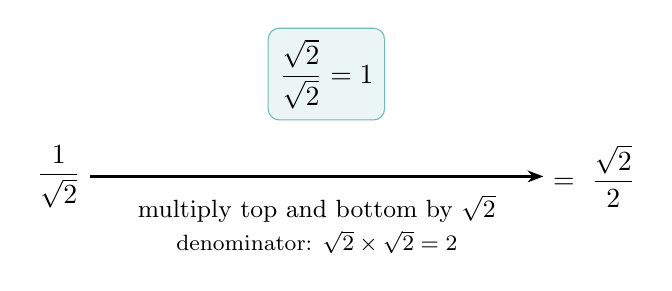
\begin{tikzpicture}[>={Stealth[length=2mm]}]
\node[draw=teal!55,rounded corners,fill=teal!8,inner sep=4pt] (rule) at (3.4,1.3) {$\displaystyle \frac{\sqrt2}{\sqrt2}=1$};
\node (L) at (0,0) {$\displaystyle \frac{1}{\sqrt2}$};
\node (R) at (6.8,0) {$\displaystyle =\ \frac{\sqrt2}{2}$};
\draw[->,thick] (L) -- (R) node[midway,below=3pt,font=\small,align=center]{multiply top and bottom by $\sqrt2$\\[1pt]\footnotesize denominator: $\sqrt2\times\sqrt2=2$};
\end{tikzpicture}
}
\end{center}
\small Multiply by $\frac{\sqrt{a}}{\sqrt{a}}=1$: this leaves the value unchanged but clears the surd from the denominator.\normalsize

\medskip\hrule

\section*{Rationalising the Denominator 02\quad\small\texttt{(a6-002)}}
\addcontentsline{toc}{section}{Rationalising the Denominator 02 (a6-002)}
\textit{Difficulty: Foundation \quad\textbar\quad Marks: 1}

\question{Rationalise the denominator: \( \frac{1}{\sqrt{5}} \)}

\textbf{Worked solution.}

\textit{Multiply the top and bottom by \( \sqrt{5} \).}
\[\begin{gathered}
\frac{1}{\sqrt{5}} \times \frac{\sqrt{5}}{\sqrt{5}} = \frac{\sqrt{5}}{5}
\end{gathered}\]
\( \sqrt{5} \times \sqrt{5} = 5 \) on the bottom, so the surd disappears.

\begin{answerbox}
\textbf{Final answer:}\quad \(\displaystyle \frac{\sqrt{5}}{5}\)
\end{answerbox}
\textbf{Diagram.}

\begin{center}
\resizebox{\ifdim\width>\linewidth \linewidth\else \width\fi}{!}{%
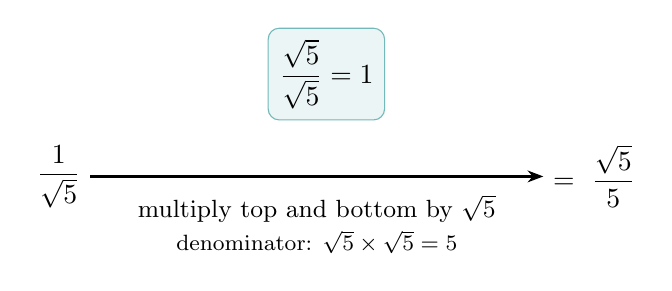
\begin{tikzpicture}[>={Stealth[length=2mm]}]
\node[draw=teal!55,rounded corners,fill=teal!8,inner sep=4pt] (rule) at (3.4,1.3) {$\displaystyle \frac{\sqrt5}{\sqrt5}=1$};
\node (L) at (0,0) {$\displaystyle \frac{1}{\sqrt5}$};
\node (R) at (6.8,0) {$\displaystyle =\ \frac{\sqrt5}{5}$};
\draw[->,thick] (L) -- (R) node[midway,below=3pt,font=\small,align=center]{multiply top and bottom by $\sqrt5$\\[1pt]\footnotesize denominator: $\sqrt5\times\sqrt5=5$};
\end{tikzpicture}
}
\end{center}
\small Multiply by $\frac{\sqrt{a}}{\sqrt{a}}=1$: this leaves the value unchanged but clears the surd from the denominator.\normalsize

\medskip\hrule

\section*{Rationalising the Denominator 03\quad\small\texttt{(a6-003)}}
\addcontentsline{toc}{section}{Rationalising the Denominator 03 (a6-003)}
\textit{Difficulty: Foundation \quad\textbar\quad Marks: 2}

\question{Simplify, giving your answer in the form \( p\sqrt{q} \) where \( p \) and \( q \) are integers: \( \frac{8}{\sqrt{2}} \)}

\textbf{Worked solution.}

\textit{Step 1: Multiply the top and bottom by \( \sqrt{2} \).}
\[\begin{gathered}
\frac{8}{\sqrt{2}} \times \frac{\sqrt{2}}{\sqrt{2}} = \frac{8\sqrt{2}}{2}
\end{gathered}\]
\( \sqrt{2} \times \sqrt{2} = 2 \).

\textit{Step 2: Simplify the fraction.}
\[\begin{gathered}
\frac{8\sqrt{2}}{2} = 4\sqrt{2}
\end{gathered}\]
Divide top and bottom by 2.

\begin{answerbox}
\textbf{Final answer:}\quad \(\displaystyle 4\sqrt{2}\)
\end{answerbox}
\textbf{Diagram.}

\begin{center}
\resizebox{\ifdim\width>\linewidth \linewidth\else \width\fi}{!}{%
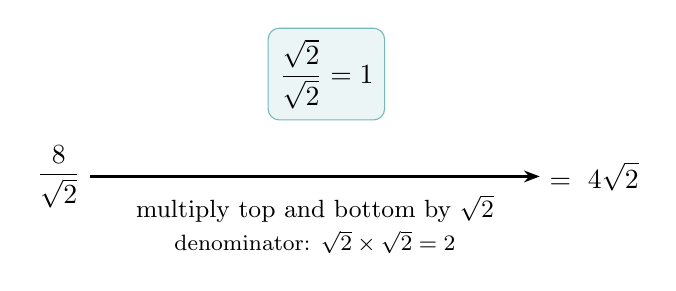
\begin{tikzpicture}[>={Stealth[length=2mm]}]
\node[draw=teal!55,rounded corners,fill=teal!8,inner sep=4pt] (rule) at (3.4,1.3) {$\displaystyle \frac{\sqrt2}{\sqrt2}=1$};
\node (L) at (0,0) {$\displaystyle \frac{8}{\sqrt2}$};
\node (R) at (6.8,0) {$\displaystyle =\ 4\sqrt2$};
\draw[->,thick] (L) -- (R) node[midway,below=3pt,font=\small,align=center]{multiply top and bottom by $\sqrt2$\\[1pt]\footnotesize denominator: $\sqrt2\times\sqrt2=2$};
\end{tikzpicture}
}
\end{center}
\small Then $\frac{8\sqrt2}{2}=4\sqrt2$. Multiply by $\frac{\sqrt{a}}{\sqrt{a}}=1$: this leaves the value unchanged but clears the surd from the denominator.\normalsize

\medskip\hrule

\section*{Rationalising the Denominator 04\quad\small\texttt{(a6-004)}}
\addcontentsline{toc}{section}{Rationalising the Denominator 04 (a6-004)}
\textit{Difficulty: Foundation \quad\textbar\quad Marks: 2}

\question{Simplify, giving your answer in the form \( p\sqrt{q} \) where \( p \) and \( q \) are integers: \( \frac{6}{\sqrt{3}} \)}

\textbf{Worked solution.}

\textit{Step 1: Multiply the top and bottom by \( \sqrt{3} \).}
\[\begin{gathered}
\frac{6}{\sqrt{3}} \times \frac{\sqrt{3}}{\sqrt{3}} = \frac{6\sqrt{3}}{3}
\end{gathered}\]
\( \sqrt{3} \times \sqrt{3} = 3 \).

\textit{Step 2: Simplify the fraction.}
\[\begin{gathered}
\frac{6\sqrt{3}}{3} = 2\sqrt{3}
\end{gathered}\]
Divide top and bottom by 3.

\begin{answerbox}
\textbf{Final answer:}\quad \(\displaystyle 2\sqrt{3}\)
\end{answerbox}
\textbf{Diagram.}

\begin{center}
\resizebox{\ifdim\width>\linewidth \linewidth\else \width\fi}{!}{%
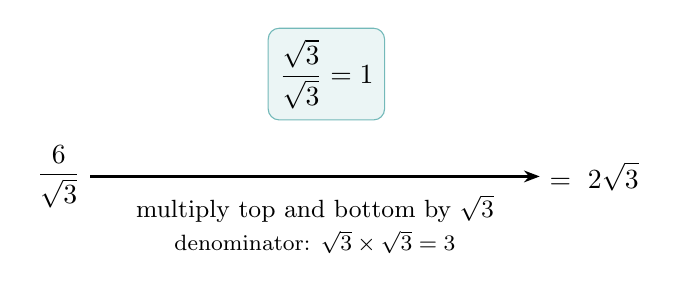
\begin{tikzpicture}[>={Stealth[length=2mm]}]
\node[draw=teal!55,rounded corners,fill=teal!8,inner sep=4pt] (rule) at (3.4,1.3) {$\displaystyle \frac{\sqrt3}{\sqrt3}=1$};
\node (L) at (0,0) {$\displaystyle \frac{6}{\sqrt3}$};
\node (R) at (6.8,0) {$\displaystyle =\ 2\sqrt3$};
\draw[->,thick] (L) -- (R) node[midway,below=3pt,font=\small,align=center]{multiply top and bottom by $\sqrt3$\\[1pt]\footnotesize denominator: $\sqrt3\times\sqrt3=3$};
\end{tikzpicture}
}
\end{center}
\small Then $\frac{6\sqrt3}{3}=2\sqrt3$. Multiply by $\frac{\sqrt{a}}{\sqrt{a}}=1$: this leaves the value unchanged but clears the surd from the denominator.\normalsize

\medskip\hrule

\section*{Rationalising the Denominator 05\quad\small\texttt{(a6-005)}}
\addcontentsline{toc}{section}{Rationalising the Denominator 05 (a6-005)}
\textit{Difficulty: Foundation \quad\textbar\quad Marks: 2}

\question{Simplify, giving your answer in the form \( p\sqrt{q} \) where \( p \) and \( q \) are integers: \( \frac{14}{\sqrt{7}} \)}

\textbf{Worked solution.}

\textit{Step 1: Multiply the top and bottom by \( \sqrt{7} \).}
\[\begin{gathered}
\frac{14}{\sqrt{7}} \times \frac{\sqrt{7}}{\sqrt{7}} = \frac{14\sqrt{7}}{7}
\end{gathered}\]
\( \sqrt{7} \times \sqrt{7} = 7 \).

\textit{Step 2: Simplify the fraction.}
\[\begin{gathered}
\frac{14\sqrt{7}}{7} = 2\sqrt{7}
\end{gathered}\]
\( 14 \div 7 = 2 \).

\begin{answerbox}
\textbf{Final answer:}\quad \(\displaystyle 2\sqrt{7}\)
\end{answerbox}
\textbf{Diagram.}

\begin{center}
\resizebox{\ifdim\width>\linewidth \linewidth\else \width\fi}{!}{%
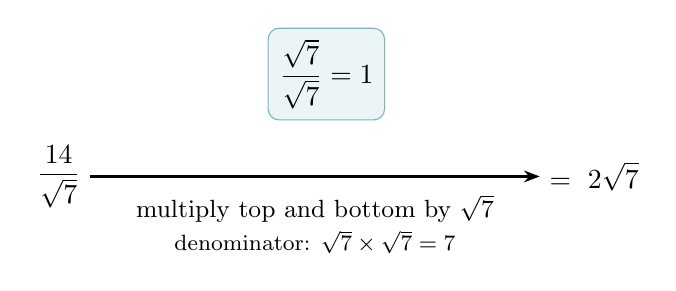
\begin{tikzpicture}[>={Stealth[length=2mm]}]
\node[draw=teal!55,rounded corners,fill=teal!8,inner sep=4pt] (rule) at (3.4,1.3) {$\displaystyle \frac{\sqrt7}{\sqrt7}=1$};
\node (L) at (0,0) {$\displaystyle \frac{14}{\sqrt7}$};
\node (R) at (6.8,0) {$\displaystyle =\ 2\sqrt7$};
\draw[->,thick] (L) -- (R) node[midway,below=3pt,font=\small,align=center]{multiply top and bottom by $\sqrt7$\\[1pt]\footnotesize denominator: $\sqrt7\times\sqrt7=7$};
\end{tikzpicture}
}
\end{center}
\small Then $\frac{14\sqrt7}{7}=2\sqrt7$. Multiply by $\frac{\sqrt{a}}{\sqrt{a}}=1$: this leaves the value unchanged but clears the surd from the denominator.\normalsize

\medskip\hrule

\section*{Rationalising the Denominator 06\quad\small\texttt{(a6-006)}}
\addcontentsline{toc}{section}{Rationalising the Denominator 06 (a6-006)}
\textit{Difficulty: Foundation \quad\textbar\quad Marks: 2}

\question{Simplify, giving your answer in the form \( p\sqrt{q} \) where \( p \) and \( q \) are integers: \( \frac{20}{\sqrt{5}} \)}

\textbf{Worked solution.}

\textit{Step 1: Multiply the top and bottom by \( \sqrt{5} \).}
\[\begin{gathered}
\frac{20}{\sqrt{5}} \times \frac{\sqrt{5}}{\sqrt{5}} = \frac{20\sqrt{5}}{5}
\end{gathered}\]
\( \sqrt{5} \times \sqrt{5} = 5 \).

\textit{Step 2: Simplify the fraction.}
\[\begin{gathered}
\frac{20\sqrt{5}}{5} = 4\sqrt{5}
\end{gathered}\]
\( 20 \div 5 = 4 \).

\begin{answerbox}
\textbf{Final answer:}\quad \(\displaystyle 4\sqrt{5}\)
\end{answerbox}
\textbf{Diagram.}

\begin{center}
\resizebox{\ifdim\width>\linewidth \linewidth\else \width\fi}{!}{%
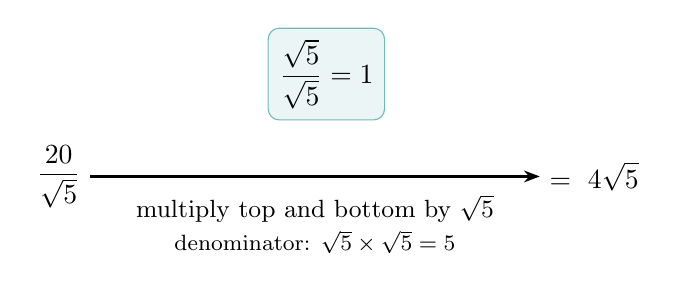
\begin{tikzpicture}[>={Stealth[length=2mm]}]
\node[draw=teal!55,rounded corners,fill=teal!8,inner sep=4pt] (rule) at (3.4,1.3) {$\displaystyle \frac{\sqrt5}{\sqrt5}=1$};
\node (L) at (0,0) {$\displaystyle \frac{20}{\sqrt5}$};
\node (R) at (6.8,0) {$\displaystyle =\ 4\sqrt5$};
\draw[->,thick] (L) -- (R) node[midway,below=3pt,font=\small,align=center]{multiply top and bottom by $\sqrt5$\\[1pt]\footnotesize denominator: $\sqrt5\times\sqrt5=5$};
\end{tikzpicture}
}
\end{center}
\small Then $\frac{20\sqrt5}{5}=4\sqrt5$. Multiply by $\frac{\sqrt{a}}{\sqrt{a}}=1$: this leaves the value unchanged but clears the surd from the denominator.\normalsize

\medskip\hrule

\section*{Rationalising the Denominator 07\quad\small\texttt{(a6-007)}}
\addcontentsline{toc}{section}{Rationalising the Denominator 07 (a6-007)}
\textit{Difficulty: Foundation \quad\textbar\quad Marks: 2}

\question{Simplify, giving your answer in the form \( p\sqrt{q} \) where \( p \) and \( q \) are integers: \( \frac{9}{\sqrt{3}} \)}

\textbf{Worked solution.}

\textit{Step 1: Multiply the top and bottom by \( \sqrt{3} \).}
\[\begin{gathered}
\frac{9}{\sqrt{3}} \times \frac{\sqrt{3}}{\sqrt{3}} = \frac{9\sqrt{3}}{3}
\end{gathered}\]
\( \sqrt{3} \times \sqrt{3} = 3 \).

\textit{Step 2: Simplify the fraction.}
\[\begin{gathered}
\frac{9\sqrt{3}}{3} = 3\sqrt{3}
\end{gathered}\]
\( 9 \div 3 = 3 \).

\begin{answerbox}
\textbf{Final answer:}\quad \(\displaystyle 3\sqrt{3}\)
\end{answerbox}
\textbf{Diagram.}

\begin{center}
\resizebox{\ifdim\width>\linewidth \linewidth\else \width\fi}{!}{%
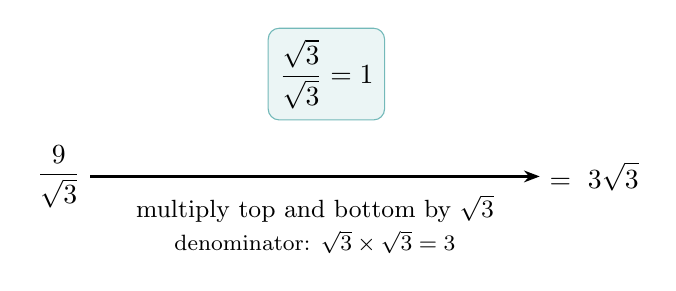
\begin{tikzpicture}[>={Stealth[length=2mm]}]
\node[draw=teal!55,rounded corners,fill=teal!8,inner sep=4pt] (rule) at (3.4,1.3) {$\displaystyle \frac{\sqrt3}{\sqrt3}=1$};
\node (L) at (0,0) {$\displaystyle \frac{9}{\sqrt3}$};
\node (R) at (6.8,0) {$\displaystyle =\ 3\sqrt3$};
\draw[->,thick] (L) -- (R) node[midway,below=3pt,font=\small,align=center]{multiply top and bottom by $\sqrt3$\\[1pt]\footnotesize denominator: $\sqrt3\times\sqrt3=3$};
\end{tikzpicture}
}
\end{center}
\small Then $\frac{9\sqrt3}{3}=3\sqrt3$. Multiply by $\frac{\sqrt{a}}{\sqrt{a}}=1$: this leaves the value unchanged but clears the surd from the denominator.\normalsize

\medskip\hrule

\section*{Rationalising the Denominator 08\quad\small\texttt{(a6-008)}}
\addcontentsline{toc}{section}{Rationalising the Denominator 08 (a6-008)}
\textit{Difficulty: Foundation \quad\textbar\quad Marks: 2}

\question{Simplify, giving your answer in the form \( p\sqrt{q} \) where \( p \) and \( q \) are integers: \( \frac{10}{\sqrt{2}} \)}

\textbf{Worked solution.}

\textit{Step 1: Multiply the top and bottom by \( \sqrt{2} \).}
\[\begin{gathered}
\frac{10}{\sqrt{2}} \times \frac{\sqrt{2}}{\sqrt{2}} = \frac{10\sqrt{2}}{2}
\end{gathered}\]
\( \sqrt{2} \times \sqrt{2} = 2 \).

\textit{Step 2: Simplify.}
\[\begin{gathered}
5\sqrt{2}
\end{gathered}\]
\( 10 \div 2 = 5 \).

\begin{answerbox}
\textbf{Final answer:}\quad \(\displaystyle 5\sqrt{2}\)
\end{answerbox}
\textbf{Diagram.}

\begin{center}
\resizebox{\ifdim\width>\linewidth \linewidth\else \width\fi}{!}{%
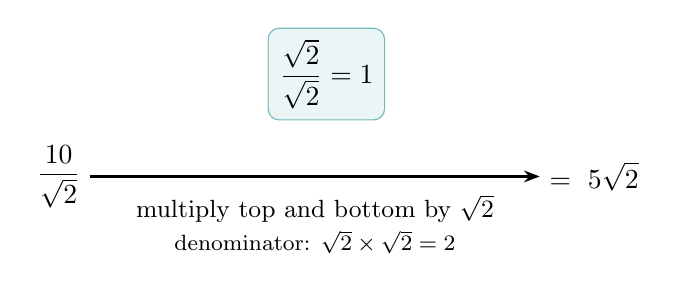
\begin{tikzpicture}[>={Stealth[length=2mm]}]
\node[draw=teal!55,rounded corners,fill=teal!8,inner sep=4pt] (rule) at (3.4,1.3) {$\displaystyle \frac{\sqrt2}{\sqrt2}=1$};
\node (L) at (0,0) {$\displaystyle \frac{10}{\sqrt2}$};
\node (R) at (6.8,0) {$\displaystyle =\ 5\sqrt2$};
\draw[->,thick] (L) -- (R) node[midway,below=3pt,font=\small,align=center]{multiply top and bottom by $\sqrt2$\\[1pt]\footnotesize denominator: $\sqrt2\times\sqrt2=2$};
\end{tikzpicture}
}
\end{center}
\small Then $\frac{10\sqrt2}{2}=5\sqrt2$. Multiply by $\frac{\sqrt{a}}{\sqrt{a}}=1$: this leaves the value unchanged but clears the surd from the denominator.\normalsize

\medskip\hrule

\section*{Rationalising the Denominator 09\quad\small\texttt{(a6-009)}}
\addcontentsline{toc}{section}{Rationalising the Denominator 09 (a6-009)}
\textit{Difficulty: Foundation \quad\textbar\quad Marks: 2}

\question{Simplify, giving your answer in the form \( p\sqrt{q} \) where \( p \) and \( q \) are integers: \( \frac{24}{\sqrt{6}} \)}

\textbf{Worked solution.}

\textit{Step 1: Multiply the top and bottom by \( \sqrt{6} \).}
\[\begin{gathered}
\frac{24\sqrt{6}}{6}
\end{gathered}\]
\( \sqrt{6} \times \sqrt{6} = 6 \).

\textit{Step 2: Simplify.}
\[\begin{gathered}
4\sqrt{6}
\end{gathered}\]
\( 24 \div 6 = 4 \).

\begin{answerbox}
\textbf{Final answer:}\quad \(\displaystyle 4\sqrt{6}\)
\end{answerbox}
\textbf{Diagram.}

\begin{center}
\resizebox{\ifdim\width>\linewidth \linewidth\else \width\fi}{!}{%
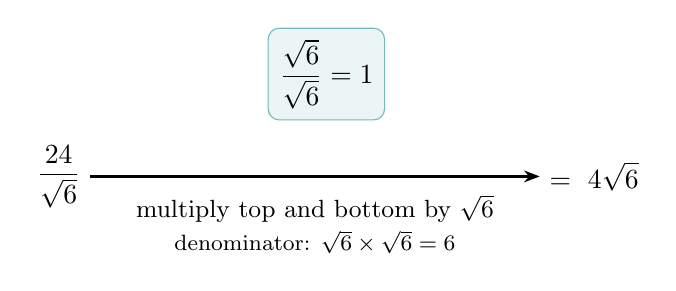
\begin{tikzpicture}[>={Stealth[length=2mm]}]
\node[draw=teal!55,rounded corners,fill=teal!8,inner sep=4pt] (rule) at (3.4,1.3) {$\displaystyle \frac{\sqrt6}{\sqrt6}=1$};
\node (L) at (0,0) {$\displaystyle \frac{24}{\sqrt6}$};
\node (R) at (6.8,0) {$\displaystyle =\ 4\sqrt6$};
\draw[->,thick] (L) -- (R) node[midway,below=3pt,font=\small,align=center]{multiply top and bottom by $\sqrt6$\\[1pt]\footnotesize denominator: $\sqrt6\times\sqrt6=6$};
\end{tikzpicture}
}
\end{center}
\small Then $\frac{24\sqrt6}{6}=4\sqrt6$. Multiply by $\frac{\sqrt{a}}{\sqrt{a}}=1$: this leaves the value unchanged but clears the surd from the denominator.\normalsize

\medskip\hrule

\section*{Rationalising the Denominator 10\quad\small\texttt{(a6-010)}}
\addcontentsline{toc}{section}{Rationalising the Denominator 10 (a6-010)}
\textit{Difficulty: Foundation \quad\textbar\quad Marks: 2}

\question{Simplify, giving your answer in the form \( p\sqrt{q} \) where \( p \) and \( q \) are integers: \( \frac{15}{\sqrt{5}} \)}

\textbf{Worked solution.}

\textit{Step 1: Multiply the top and bottom by \( \sqrt{5} \).}
\[\begin{gathered}
\frac{15\sqrt{5}}{5}
\end{gathered}\]
\( \sqrt{5} \times \sqrt{5} = 5 \).

\textit{Step 2: Simplify.}
\[\begin{gathered}
3\sqrt{5}
\end{gathered}\]
\( 15 \div 5 = 3 \).

\begin{answerbox}
\textbf{Final answer:}\quad \(\displaystyle 3\sqrt{5}\)
\end{answerbox}
\textbf{Diagram.}

\begin{center}
\resizebox{\ifdim\width>\linewidth \linewidth\else \width\fi}{!}{%
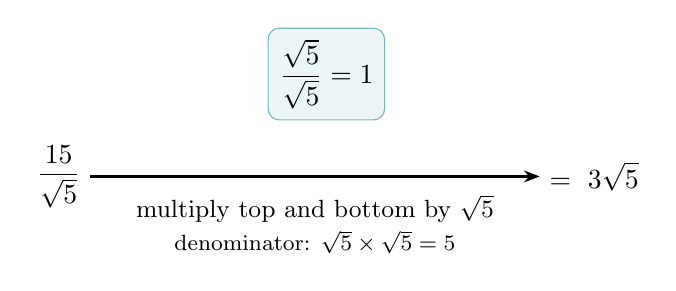
\begin{tikzpicture}[>={Stealth[length=2mm]}]
\node[draw=teal!55,rounded corners,fill=teal!8,inner sep=4pt] (rule) at (3.4,1.3) {$\displaystyle \frac{\sqrt5}{\sqrt5}=1$};
\node (L) at (0,0) {$\displaystyle \frac{15}{\sqrt5}$};
\node (R) at (6.8,0) {$\displaystyle =\ 3\sqrt5$};
\draw[->,thick] (L) -- (R) node[midway,below=3pt,font=\small,align=center]{multiply top and bottom by $\sqrt5$\\[1pt]\footnotesize denominator: $\sqrt5\times\sqrt5=5$};
\end{tikzpicture}
}
\end{center}
\small Then $\frac{15\sqrt5}{5}=3\sqrt5$. Multiply by $\frac{\sqrt{a}}{\sqrt{a}}=1$: this leaves the value unchanged but clears the surd from the denominator.\normalsize

\medskip\hrule

\section*{Rationalising the Denominator 11\quad\small\texttt{(a6-011)}}
\addcontentsline{toc}{section}{Rationalising the Denominator 11 (a6-011)}
\textit{Difficulty: Foundation \quad\textbar\quad Marks: 3}

\question{Simplify, giving your answer in the form \( p\sqrt{q} \) where \( p \) and \( q \) are integers: \( \sqrt{32} + \frac{10}{\sqrt{2}} \)}

\textbf{Worked solution.}

\textit{Step 1: Simplify \( \sqrt{32} \).}
\[\begin{gathered}
\sqrt{32} = \sqrt{16 \times 2} = 4\sqrt{2}
\end{gathered}\]
16 is the largest square factor of 32.

\textit{Step 2: Rationalise the second term.}
\[\begin{gathered}
\frac{10}{\sqrt{2}} = \frac{10\sqrt{2}}{2} = 5\sqrt{2}
\end{gathered}\]
Multiply top and bottom by \( \sqrt{2} \), then simplify.

\textit{Step 3: Add the like surds.}
\[\begin{gathered}
4\sqrt{2} + 5\sqrt{2} = 9\sqrt{2}
\end{gathered}\]
\( 4 + 5 = 9 \).

\begin{answerbox}
\textbf{Final answer:}\quad \(\displaystyle 9\sqrt{2}\)
\end{answerbox}
\textbf{Diagram.}

\begin{center}
\resizebox{\ifdim\width>\linewidth \linewidth\else \width\fi}{!}{%
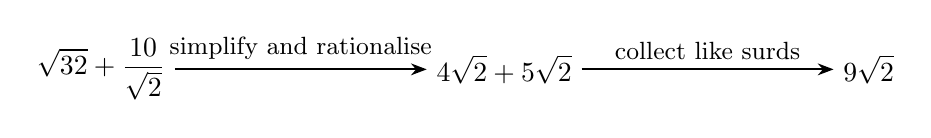
\begin{tikzpicture}[>={Stealth[length=2mm]},node distance=1.5cm and 3.2cm]
\node (s0) {$\displaystyle \sqrt{32}+\frac{10}{\sqrt2}$};
\node (s1) [right=of s0] {$\displaystyle 4\sqrt2+5\sqrt2$};
\node (s2) [right=of s1] {$\displaystyle 9\sqrt2$};
\draw[->,thick] (s0) -- (s1) node[midway,above,font=\small]{simplify and rationalise};
\draw[->,thick] (s1) -- (s2) node[midway,above,font=\small]{collect like surds};
\end{tikzpicture}
}
\end{center}
\small Solution flow: each arrow applies one step.\normalsize

\medskip\hrule

\section*{Rationalising the Denominator 12\quad\small\texttt{(a6-012)}}
\addcontentsline{toc}{section}{Rationalising the Denominator 12 (a6-012)}
\textit{Difficulty: Foundation \quad\textbar\quad Marks: 3}

\question{Simplify, giving your answer in the form \( p\sqrt{q} \) where \( p \) and \( q \) are integers: \( \sqrt{75} - \frac{6}{\sqrt{3}} \)}

\textbf{Worked solution.}

\textit{Step 1: Simplify \( \sqrt{75} \).}
\[\begin{gathered}
\sqrt{75} = \sqrt{25 \times 3} = 5\sqrt{3}
\end{gathered}\]
25 is the largest square factor of 75.

\textit{Step 2: Rationalise the second term.}
\[\begin{gathered}
\frac{6}{\sqrt{3}} = \frac{6\sqrt{3}}{3} = 2\sqrt{3}
\end{gathered}\]
Multiply top and bottom by \( \sqrt{3} \).

\textit{Step 3: Subtract the like surds.}
\[\begin{gathered}
5\sqrt{3} - 2\sqrt{3} = 3\sqrt{3}
\end{gathered}\]
\( 5 - 2 = 3 \).

\begin{answerbox}
\textbf{Final answer:}\quad \(\displaystyle 3\sqrt{3}\)
\end{answerbox}
\textbf{Diagram.}

\begin{center}
\resizebox{\ifdim\width>\linewidth \linewidth\else \width\fi}{!}{%
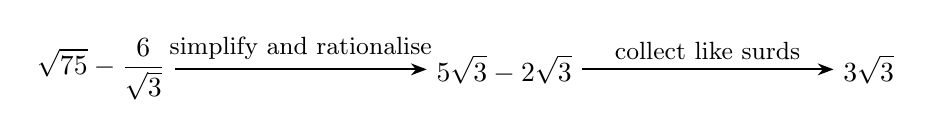
\begin{tikzpicture}[>={Stealth[length=2mm]},node distance=1.5cm and 3.2cm]
\node (s0) {$\displaystyle \sqrt{75}-\frac{6}{\sqrt3}$};
\node (s1) [right=of s0] {$\displaystyle 5\sqrt3-2\sqrt3$};
\node (s2) [right=of s1] {$\displaystyle 3\sqrt3$};
\draw[->,thick] (s0) -- (s1) node[midway,above,font=\small]{simplify and rationalise};
\draw[->,thick] (s1) -- (s2) node[midway,above,font=\small]{collect like surds};
\end{tikzpicture}
}
\end{center}
\small Solution flow: each arrow applies one step.\normalsize

\medskip\hrule

\section*{Rationalising the Denominator 13\quad\small\texttt{(a6-013)}}
\addcontentsline{toc}{section}{Rationalising the Denominator 13 (a6-013)}
\textit{Difficulty: Foundation \quad\textbar\quad Marks: 2}

\question{Rationalise the denominator: \( \frac{3}{\sqrt{6}} \)}

\textbf{Worked solution.}

\textit{Step 1: Multiply the top and bottom by \( \sqrt{6} \).}
\[\begin{gathered}
\frac{3}{\sqrt{6}} \times \frac{\sqrt{6}}{\sqrt{6}} = \frac{3\sqrt{6}}{6}
\end{gathered}\]
\( \sqrt{6} \times \sqrt{6} = 6 \).

\textit{Step 2: Simplify the fraction.}
\[\begin{gathered}
\frac{\sqrt{6}}{2}
\end{gathered}\]
Divide top and bottom by 3.

\begin{answerbox}
\textbf{Final answer:}\quad \(\displaystyle \frac{\sqrt{6}}{2}\)
\end{answerbox}
\textbf{Diagram.}

\begin{center}
\resizebox{\ifdim\width>\linewidth \linewidth\else \width\fi}{!}{%
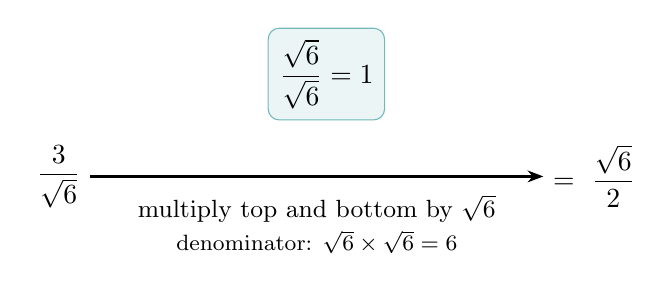
\begin{tikzpicture}[>={Stealth[length=2mm]}]
\node[draw=teal!55,rounded corners,fill=teal!8,inner sep=4pt] (rule) at (3.4,1.3) {$\displaystyle \frac{\sqrt6}{\sqrt6}=1$};
\node (L) at (0,0) {$\displaystyle \frac{3}{\sqrt6}$};
\node (R) at (6.8,0) {$\displaystyle =\ \frac{\sqrt6}{2}$};
\draw[->,thick] (L) -- (R) node[midway,below=3pt,font=\small,align=center]{multiply top and bottom by $\sqrt6$\\[1pt]\footnotesize denominator: $\sqrt6\times\sqrt6=6$};
\end{tikzpicture}
}
\end{center}
\small Then $\frac{3\sqrt6}{6}=\frac{\sqrt6}{2}$. Multiply by $\frac{\sqrt{a}}{\sqrt{a}}=1$: this leaves the value unchanged but clears the surd from the denominator.\normalsize

\medskip\hrule

\section*{Rationalising the Denominator 14\quad\small\texttt{(a6-014)}}
\addcontentsline{toc}{section}{Rationalising the Denominator 14 (a6-014)}
\textit{Difficulty: Foundation \quad\textbar\quad Marks: 2}

\question{Rationalise the denominator: \( \frac{4}{\sqrt{10}} \)}

\textbf{Worked solution.}

\textit{Step 1: Multiply the top and bottom by \( \sqrt{10} \).}
\[\begin{gathered}
\frac{4\sqrt{10}}{10}
\end{gathered}\]
\( \sqrt{10} \times \sqrt{10} = 10 \).

\textit{Step 2: Simplify by dividing top and bottom by 2.}
\[\begin{gathered}
\frac{2\sqrt{10}}{5}
\end{gathered}\]
The 4 and the 10 share a common factor of 2.

\begin{answerbox}
\textbf{Final answer:}\quad \(\displaystyle \frac{2\sqrt{10}}{5}\)
\end{answerbox}
\textbf{Diagram.}

\begin{center}
\resizebox{\ifdim\width>\linewidth \linewidth\else \width\fi}{!}{%
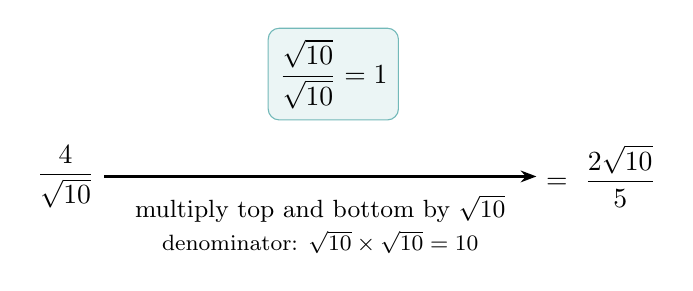
\begin{tikzpicture}[>={Stealth[length=2mm]}]
\node[draw=teal!55,rounded corners,fill=teal!8,inner sep=4pt] (rule) at (3.4,1.3) {$\displaystyle \frac{\sqrt{10}}{\sqrt{10}}=1$};
\node (L) at (0,0) {$\displaystyle \frac{4}{\sqrt{10}}$};
\node (R) at (6.8,0) {$\displaystyle =\ \frac{2\sqrt{10}}{5}$};
\draw[->,thick] (L) -- (R) node[midway,below=3pt,font=\small,align=center]{multiply top and bottom by $\sqrt{10}$\\[1pt]\footnotesize denominator: $\sqrt{10}\times\sqrt{10}=10$};
\end{tikzpicture}
}
\end{center}
\small Then $\frac{4\sqrt{10}}{10}=\frac{2\sqrt{10}}{5}$. Multiply by $\frac{\sqrt{a}}{\sqrt{a}}=1$: this leaves the value unchanged but clears the surd from the denominator.\normalsize

\medskip\hrule

\section*{Rationalising the Denominator 15\quad\small\texttt{(a6-015)}}
\addcontentsline{toc}{section}{Rationalising the Denominator 15 (a6-015)}
\textit{Difficulty: Foundation \quad\textbar\quad Marks: 3}

\question{Rationalise the denominator: \( \frac{\sqrt{3}}{\sqrt{8}} \)}

\textbf{Worked solution.}

\textit{Step 1: Simplify \( \sqrt{8} \) first.}
\[\begin{gathered}
\frac{\sqrt{3}}{\sqrt{8}} = \frac{\sqrt{3}}{2\sqrt{2}}
\end{gathered}\]
\( \sqrt{8} = \sqrt{4 \times 2} = 2\sqrt{2} \).

\textit{Step 2: Multiply the top and bottom by \( \sqrt{2} \).}
\[\begin{gathered}
\frac{\sqrt{3} \times \sqrt{2}}{2\sqrt{2} \times \sqrt{2}} = \frac{\sqrt{6}}{4}
\end{gathered}\]
\( \sqrt{3} \times \sqrt{2} = \sqrt{6} \) and \( 2\sqrt{2} \times \sqrt{2} = 2 \times 2 = 4 \).

\begin{answerbox}
\textbf{Final answer:}\quad \(\displaystyle \frac{\sqrt{6}}{4}\)
\end{answerbox}
\textbf{Diagram.}

\begin{center}
\resizebox{\ifdim\width>\linewidth \linewidth\else \width\fi}{!}{%
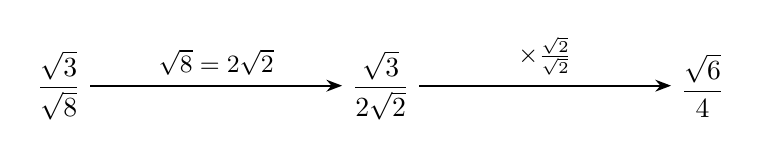
\begin{tikzpicture}[>={Stealth[length=2mm]},node distance=1.5cm and 3.2cm]
\node (s0) {$\displaystyle \frac{\sqrt3}{\sqrt8}$};
\node (s1) [right=of s0] {$\displaystyle \frac{\sqrt3}{2\sqrt2}$};
\node (s2) [right=of s1] {$\displaystyle \frac{\sqrt6}{4}$};
\draw[->,thick] (s0) -- (s1) node[midway,above,font=\small]{$\sqrt8=2\sqrt2$};
\draw[->,thick] (s1) -- (s2) node[midway,above,font=\small]{$\times\tfrac{\sqrt2}{\sqrt2}$};
\end{tikzpicture}
}
\end{center}
\small Solution flow: each arrow applies one step.\normalsize

\medskip\hrule

\section*{Rationalising the Denominator 16\quad\small\texttt{(a6-016)}}
\addcontentsline{toc}{section}{Rationalising the Denominator 16 (a6-016)}
\textit{Difficulty: Foundation \quad\textbar\quad Marks: 2}

\question{Rationalise the denominator: \( \frac{5}{2\sqrt{3}} \)}

\textbf{Worked solution.}

\textit{Step 1: Multiply the top and bottom by \( \sqrt{3} \).}
\[\begin{gathered}
\frac{5}{2\sqrt{3}} \times \frac{\sqrt{3}}{\sqrt{3}} = \frac{5\sqrt{3}}{2 \times 3}
\end{gathered}\]
\( 2\sqrt{3} \times \sqrt{3} = 2 \times 3 = 6 \).

\textit{Step 2: Write the final answer.}
\[\begin{gathered}
\frac{5\sqrt{3}}{6}
\end{gathered}\]
\( \frac{5\sqrt{3}}{6} \) cannot be simplified further.

\begin{answerbox}
\textbf{Final answer:}\quad \(\displaystyle \frac{5\sqrt{3}}{6}\)
\end{answerbox}
\textbf{Diagram.}

\begin{center}
\resizebox{\ifdim\width>\linewidth \linewidth\else \width\fi}{!}{%
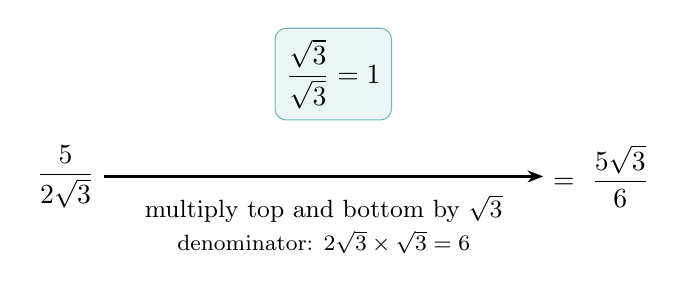
\begin{tikzpicture}[>={Stealth[length=2mm]}]
\node[draw=teal!55,rounded corners,fill=teal!8,inner sep=4pt] (rule) at (3.4,1.3) {$\displaystyle \frac{\sqrt3}{\sqrt3}=1$};
\node (L) at (0,0) {$\displaystyle \frac{5}{2\sqrt3}$};
\node (R) at (6.8,0) {$\displaystyle =\ \frac{5\sqrt3}{6}$};
\draw[->,thick] (L) -- (R) node[midway,below=3pt,font=\small,align=center]{multiply top and bottom by $\sqrt3$\\[1pt]\footnotesize denominator: $2\sqrt3\times\sqrt3=6$};
\end{tikzpicture}
}
\end{center}
\small Multiply by $\frac{\sqrt{a}}{\sqrt{a}}=1$: this leaves the value unchanged but clears the surd from the denominator.\normalsize

\medskip\hrule

\section*{Rationalising the Denominator 17\quad\small\texttt{(a6-017)}}
\addcontentsline{toc}{section}{Rationalising the Denominator 17 (a6-017)}
\textit{Difficulty: Foundation \quad\textbar\quad Marks: 2}

\question{Rationalise the denominator and simplify: \( \frac{\sqrt{18}}{\sqrt{2}} \)}

\textbf{Worked solution.}

\textit{Step 1: Use the rule \( \frac{\sqrt{a}}{\sqrt{b}} = \sqrt{\frac{a}{b}} \).}
\[\begin{gathered}
\sqrt{\frac{18}{2}} = \sqrt{9}
\end{gathered}\]
When dividing surds with the same type, you can combine them under a single root sign.

\textit{Step 2: Evaluate.}
\[\begin{gathered}
3
\end{gathered}\]
\( \sqrt{9} = 3 \). The answer is a whole number — no surds remain.

\begin{answerbox}
\textbf{Final answer:}\quad \(\displaystyle 3\)
\end{answerbox}
\textbf{Diagram.}

\begin{center}
\resizebox{\ifdim\width>\linewidth \linewidth\else \width\fi}{!}{%
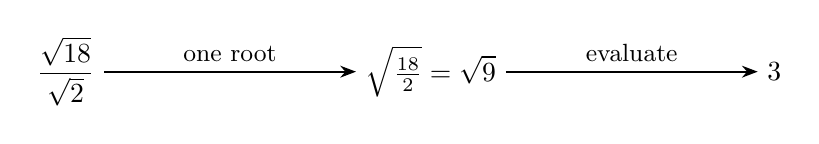
\begin{tikzpicture}[>={Stealth[length=2mm]},node distance=1.5cm and 3.2cm]
\node (s0) {$\displaystyle \frac{\sqrt{18}}{\sqrt2}$};
\node (s1) [right=of s0] {$\displaystyle \sqrt{\tfrac{18}{2}}=\sqrt9$};
\node (s2) [right=of s1] {$\displaystyle 3$};
\draw[->,thick] (s0) -- (s1) node[midway,above,font=\small]{one root};
\draw[->,thick] (s1) -- (s2) node[midway,above,font=\small]{evaluate};
\end{tikzpicture}
}
\end{center}
\small Solution flow: each arrow applies one step.\normalsize

\medskip\hrule

\section*{Rationalising the Denominator 18\quad\small\texttt{(a6-018)}}
\addcontentsline{toc}{section}{Rationalising the Denominator 18 (a6-018)}
\textit{Difficulty: Foundation \quad\textbar\quad Marks: 3}

\question{Express in the form \( a + b\sqrt{k} \) where \( a \), \( b \) and \( k \) are integers: \( \frac{2}{1 + \sqrt{3}} \)}

\textbf{Worked solution.}

\textit{Step 1: Multiply the top and bottom by the conjugate \( 1 - \sqrt{3} \).}
\[\begin{gathered}
\frac{2}{1 + \sqrt{3}} \times \frac{1 - \sqrt{3}}{1 - \sqrt{3}} = \frac{2(1 - \sqrt{3})}{(1 + \sqrt{3})(1 - \sqrt{3})}
\end{gathered}\]
The conjugate has the opposite sign between the terms. Multiplying by it removes the surd from the denominator.

\textit{Step 2: Expand the denominator using the difference of two squares.}
\[\begin{gathered}
\frac{2(1 - \sqrt{3})}{1 - 3} = \frac{2(1 - \sqrt{3})}{-2}
\end{gathered}\]
\( (1 + \sqrt{3})(1 - \sqrt{3}) = 1 - 3 = -2 \).

\textit{Step 3: Cancel and simplify.}
\[\begin{gathered}
-(1 - \sqrt{3}) = -1 + \sqrt{3}
\end{gathered}\]
Dividing by \( -2 \): \( \frac{2}{-2} = -1 \). So \( a = -1 \), \( b = 1 \), \( k = 3 \).

\begin{answerbox}
\textbf{Final answer:}\quad \(\displaystyle -1 + \sqrt{3}\)
\end{answerbox}
\textbf{Diagram.}

\begin{center}
\resizebox{\ifdim\width>\linewidth \linewidth\else \width\fi}{!}{%
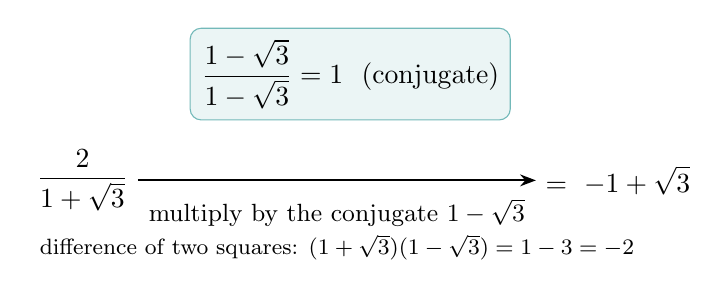
\begin{tikzpicture}[>={Stealth[length=2mm]}]
\node[draw=teal!55,rounded corners,fill=teal!8,inner sep=4pt] (rule) at (3.4,1.35) {$\displaystyle \frac{1-\sqrt3}{1-\sqrt3}=1$ \ (conjugate)};
\node (L) at (0,0) {$\displaystyle \frac{2}{1+\sqrt3}$};
\node (R) at (6.8,0) {$\displaystyle =\ -1+\sqrt3$};
\draw[->,thick] (L) -- (R) node[midway,below=3pt,font=\small,align=center]{multiply by the conjugate $1-\sqrt3$\\[1pt]\footnotesize difference of two squares: $(1+\sqrt3)(1-\sqrt3)=1-3=-2$};
\end{tikzpicture}
}
\end{center}
\small Multiply by the conjugate over itself. The denominator is then a difference of two squares, $(A+B)(A-B)=A^{2}-B^{2}$, so every surd cancels and the denominator becomes rational.\normalsize

\medskip\hrule

\section*{Rationalising the Denominator 19\quad\small\texttt{(a6-019)}}
\addcontentsline{toc}{section}{Rationalising the Denominator 19 (a6-019)}
\textit{Difficulty: Foundation \quad\textbar\quad Marks: 3}

\question{Express in the form \( a + b\sqrt{k} \) where \( a \), \( b \) and \( k \) are integers: \( \frac{8}{\sqrt{5} - 1} \)}

\textbf{Worked solution.}

\textit{Step 1: Multiply the top and bottom by the conjugate \( \sqrt{5} + 1 \).}
\[\begin{gathered}
\frac{8(\sqrt{5} + 1)}{(\sqrt{5} - 1)(\sqrt{5} + 1)}
\end{gathered}\]
The conjugate of \( \sqrt{5} - 1 \) is \( \sqrt{5} + 1 \).

\textit{Step 2: Expand the denominator using the difference of two squares.}
\[\begin{gathered}
\frac{8(\sqrt{5} + 1)}{5 - 1} = \frac{8(\sqrt{5} + 1)}{4}
\end{gathered}\]
\( (\sqrt{5})^2 - 1^2 = 5 - 1 = 4 \).

\textit{Step 3: Divide the numerator by 4.}
\[\begin{gathered}
2(\sqrt{5} + 1) = 2 + 2\sqrt{5}
\end{gathered}\]
Since 8 ÷ 4 = 2, we get integer coefficients \( a = 2 \), \( b = 2 \), \( k = 5 \).

\begin{answerbox}
\textbf{Final answer:}\quad \(\displaystyle 2 + 2\sqrt{5}\)
\end{answerbox}
\textbf{Diagram.}

\begin{center}
\resizebox{\ifdim\width>\linewidth \linewidth\else \width\fi}{!}{%
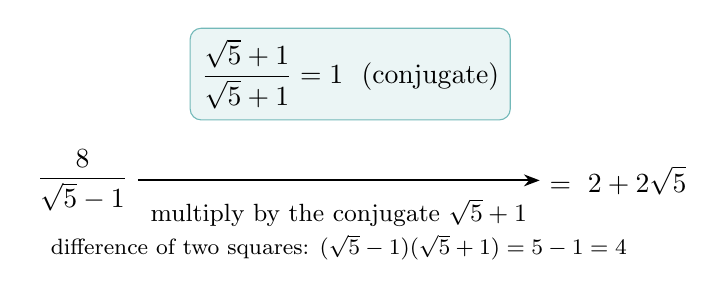
\begin{tikzpicture}[>={Stealth[length=2mm]}]
\node[draw=teal!55,rounded corners,fill=teal!8,inner sep=4pt] (rule) at (3.4,1.35) {$\displaystyle \frac{\sqrt5+1}{\sqrt5+1}=1$ \ (conjugate)};
\node (L) at (0,0) {$\displaystyle \frac{8}{\sqrt5-1}$};
\node (R) at (6.8,0) {$\displaystyle =\ 2+2\sqrt5$};
\draw[->,thick] (L) -- (R) node[midway,below=3pt,font=\small,align=center]{multiply by the conjugate $\sqrt5+1$\\[1pt]\footnotesize difference of two squares: $(\sqrt5-1)(\sqrt5+1)=5-1=4$};
\end{tikzpicture}
}
\end{center}
\small Multiply by the conjugate over itself. The denominator is then a difference of two squares, $(A+B)(A-B)=A^{2}-B^{2}$, so every surd cancels and the denominator becomes rational.\normalsize

\medskip\hrule

\section*{Rationalising the Denominator 20\quad\small\texttt{(a6-020)}}
\addcontentsline{toc}{section}{Rationalising the Denominator 20 (a6-020)}
\textit{Difficulty: Foundation \quad\textbar\quad Marks: 3}

\question{Express in the form \( a + b\sqrt{k} \) where \( a \), \( b \) and \( k \) are integers: \( \frac{7}{3 - \sqrt{2}} \)}

\textbf{Worked solution.}

\textit{Step 1: Multiply the top and bottom by the conjugate \( 3 + \sqrt{2} \).}
\[\begin{gathered}
\frac{7(3 + \sqrt{2})}{(3 - \sqrt{2})(3 + \sqrt{2})}
\end{gathered}\]
The conjugate flips the sign between the terms.

\textit{Step 2: Expand the denominator.}
\[\begin{gathered}
\frac{7(3 + \sqrt{2})}{9 - 2} = \frac{7(3 + \sqrt{2})}{7}
\end{gathered}\]
\( 3^2 - (\sqrt{2})^2 = 9 - 2 = 7 \).

\textit{Step 3: Cancel the common factor of 7.}
\[\begin{gathered}
3 + \sqrt{2}
\end{gathered}\]
The 7 in the numerator and denominator cancel, giving \( a = 3 \), \( b = 1 \), \( k = 2 \).

\begin{answerbox}
\textbf{Final answer:}\quad \(\displaystyle 3 + \sqrt{2}\)
\end{answerbox}
\textbf{Diagram.}

\begin{center}
\resizebox{\ifdim\width>\linewidth \linewidth\else \width\fi}{!}{%
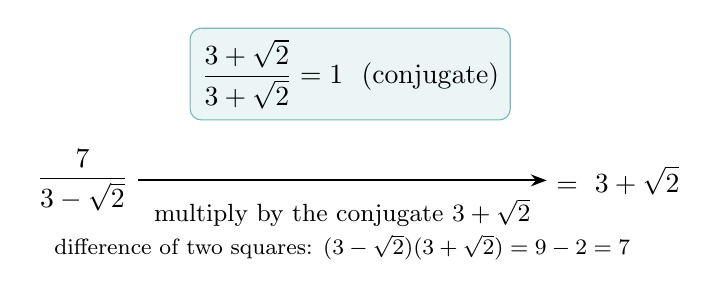
\begin{tikzpicture}[>={Stealth[length=2mm]}]
\node[draw=teal!55,rounded corners,fill=teal!8,inner sep=4pt] (rule) at (3.4,1.35) {$\displaystyle \frac{3+\sqrt2}{3+\sqrt2}=1$ \ (conjugate)};
\node (L) at (0,0) {$\displaystyle \frac{7}{3-\sqrt2}$};
\node (R) at (6.8,0) {$\displaystyle =\ 3+\sqrt2$};
\draw[->,thick] (L) -- (R) node[midway,below=3pt,font=\small,align=center]{multiply by the conjugate $3+\sqrt2$\\[1pt]\footnotesize difference of two squares: $(3-\sqrt2)(3+\sqrt2)=9-2=7$};
\end{tikzpicture}
}
\end{center}
\small Multiply by the conjugate over itself. The denominator is then a difference of two squares, $(A+B)(A-B)=A^{2}-B^{2}$, so every surd cancels and the denominator becomes rational.\normalsize

\medskip\hrule

\section*{Rationalising the Denominator 21\quad\small\texttt{(a6-021)}}
\addcontentsline{toc}{section}{Rationalising the Denominator 21 (a6-021)}
\textit{Difficulty: Foundation \quad\textbar\quad Marks: 3}

\question{Express in the form \( a + b\sqrt{k} \) where \( a \), \( b \) and \( k \) are integers: \( \frac{4}{\sqrt{6} - 2} \)}

\textbf{Worked solution.}

\textit{Step 1: Multiply the top and bottom by the conjugate \( \sqrt{6} + 2 \).}
\[\begin{gathered}
\frac{4(\sqrt{6} + 2)}{(\sqrt{6} - 2)(\sqrt{6} + 2)}
\end{gathered}\]
The conjugate has the opposite sign.

\textit{Step 2: Expand the denominator using the difference of two squares.}
\[\begin{gathered}
\frac{4(\sqrt{6} + 2)}{6 - 4} = \frac{4(\sqrt{6} + 2)}{2}
\end{gathered}\]
\( (\sqrt{6})^2 - 2^2 = 6 - 4 = 2 \).

\textit{Step 3: Divide and expand.}
\[\begin{gathered}
2(\sqrt{6} + 2) = 4 + 2\sqrt{6}
\end{gathered}\]
\( \frac{4}{2} = 2 \), then multiply through.

\begin{answerbox}
\textbf{Final answer:}\quad \(\displaystyle 4 + 2\sqrt{6}\)
\end{answerbox}
\textbf{Diagram.}

\begin{center}
\resizebox{\ifdim\width>\linewidth \linewidth\else \width\fi}{!}{%
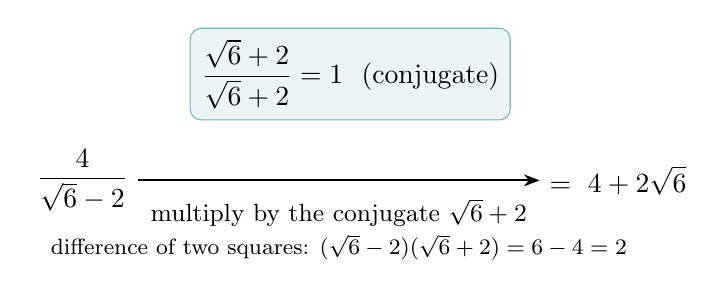
\begin{tikzpicture}[>={Stealth[length=2mm]}]
\node[draw=teal!55,rounded corners,fill=teal!8,inner sep=4pt] (rule) at (3.4,1.35) {$\displaystyle \frac{\sqrt6+2}{\sqrt6+2}=1$ \ (conjugate)};
\node (L) at (0,0) {$\displaystyle \frac{4}{\sqrt6-2}$};
\node (R) at (6.8,0) {$\displaystyle =\ 4+2\sqrt6$};
\draw[->,thick] (L) -- (R) node[midway,below=3pt,font=\small,align=center]{multiply by the conjugate $\sqrt6+2$\\[1pt]\footnotesize difference of two squares: $(\sqrt6-2)(\sqrt6+2)=6-4=2$};
\end{tikzpicture}
}
\end{center}
\small Multiply by the conjugate over itself. The denominator is then a difference of two squares, $(A+B)(A-B)=A^{2}-B^{2}$, so every surd cancels and the denominator becomes rational.\normalsize

\medskip\hrule

\section*{Rationalising the Denominator 22\quad\small\texttt{(a6-022)}}
\addcontentsline{toc}{section}{Rationalising the Denominator 22 (a6-022)}
\textit{Difficulty: Foundation \quad\textbar\quad Marks: 3}

\question{Express in the form \( a + b\sqrt{k} \) where \( a \), \( b \) and \( k \) are integers: \( \frac{14}{4 + \sqrt{2}} \)}

\textbf{Worked solution.}

\textit{Step 1: Multiply the top and bottom by the conjugate \( 4 - \sqrt{2} \).}
\[\begin{gathered}
\frac{14(4 - \sqrt{2})}{(4 + \sqrt{2})(4 - \sqrt{2})}
\end{gathered}\]
The conjugate flips the middle sign.

\textit{Step 2: Expand the denominator.}
\[\begin{gathered}
\frac{14(4 - \sqrt{2})}{16 - 2} = \frac{14(4 - \sqrt{2})}{14}
\end{gathered}\]
\( 4^2 - (\sqrt{2})^2 = 16 - 2 = 14 \).

\textit{Step 3: Cancel the 14.}
\[\begin{gathered}
4 - \sqrt{2}
\end{gathered}\]
The 14 on top and bottom cancel exactly.

\begin{answerbox}
\textbf{Final answer:}\quad \(\displaystyle 4 - \sqrt{2}\)
\end{answerbox}
\textbf{Diagram.}

\begin{center}
\resizebox{\ifdim\width>\linewidth \linewidth\else \width\fi}{!}{%
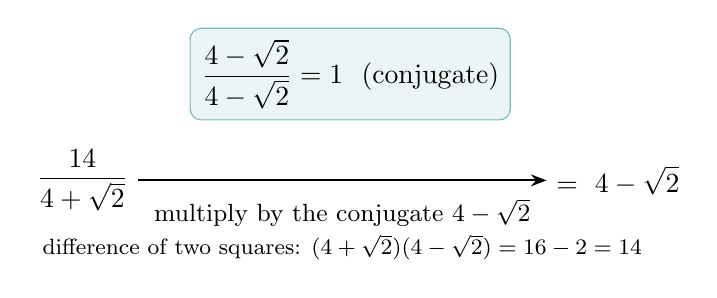
\begin{tikzpicture}[>={Stealth[length=2mm]}]
\node[draw=teal!55,rounded corners,fill=teal!8,inner sep=4pt] (rule) at (3.4,1.35) {$\displaystyle \frac{4-\sqrt2}{4-\sqrt2}=1$ \ (conjugate)};
\node (L) at (0,0) {$\displaystyle \frac{14}{4+\sqrt2}$};
\node (R) at (6.8,0) {$\displaystyle =\ 4-\sqrt2$};
\draw[->,thick] (L) -- (R) node[midway,below=3pt,font=\small,align=center]{multiply by the conjugate $4-\sqrt2$\\[1pt]\footnotesize difference of two squares: $(4+\sqrt2)(4-\sqrt2)=16-2=14$};
\end{tikzpicture}
}
\end{center}
\small Multiply by the conjugate over itself. The denominator is then a difference of two squares, $(A+B)(A-B)=A^{2}-B^{2}$, so every surd cancels and the denominator becomes rational.\normalsize

\medskip\hrule

\section*{Rationalising the Denominator 23\quad\small\texttt{(a6-023)}}
\addcontentsline{toc}{section}{Rationalising the Denominator 23 (a6-023)}
\textit{Difficulty: Foundation \quad\textbar\quad Marks: 3}

\question{Express in the form \( a + b\sqrt{k} \) where \( a \), \( b \) and \( k \) are integers: \( \frac{12}{5 - \sqrt{13}} \)}

\textbf{Worked solution.}

\textit{Step 1: Multiply the top and bottom by the conjugate \( 5 + \sqrt{13} \).}
\[\begin{gathered}
\frac{12(5 + \sqrt{13})}{(5 - \sqrt{13})(5 + \sqrt{13})}
\end{gathered}\]
Flip the sign between the terms.

\textit{Step 2: Expand the denominator.}
\[\begin{gathered}
\frac{12(5 + \sqrt{13})}{25 - 13} = \frac{12(5 + \sqrt{13})}{12}
\end{gathered}\]
\( 5^2 - (\sqrt{13})^2 = 25 - 13 = 12 \).

\textit{Step 3: Cancel the 12.}
\[\begin{gathered}
5 + \sqrt{13}
\end{gathered}\]
The 12s cancel, leaving the numerator bracket.

\begin{answerbox}
\textbf{Final answer:}\quad \(\displaystyle 5 + \sqrt{13}\)
\end{answerbox}
\textbf{Diagram.}

\begin{center}
\resizebox{\ifdim\width>\linewidth \linewidth\else \width\fi}{!}{%
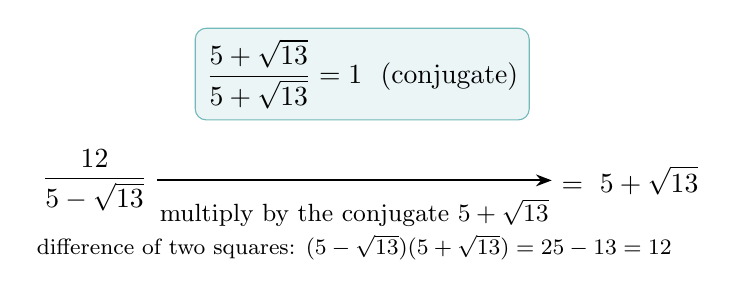
\begin{tikzpicture}[>={Stealth[length=2mm]}]
\node[draw=teal!55,rounded corners,fill=teal!8,inner sep=4pt] (rule) at (3.4,1.35) {$\displaystyle \frac{5+\sqrt{13}}{5+\sqrt{13}}=1$ \ (conjugate)};
\node (L) at (0,0) {$\displaystyle \frac{12}{5-\sqrt{13}}$};
\node (R) at (6.8,0) {$\displaystyle =\ 5+\sqrt{13}$};
\draw[->,thick] (L) -- (R) node[midway,below=3pt,font=\small,align=center]{multiply by the conjugate $5+\sqrt{13}$\\[1pt]\footnotesize difference of two squares: $(5-\sqrt{13})(5+\sqrt{13})=25-13=12$};
\end{tikzpicture}
}
\end{center}
\small Multiply by the conjugate over itself. The denominator is then a difference of two squares, $(A+B)(A-B)=A^{2}-B^{2}$, so every surd cancels and the denominator becomes rational.\normalsize

\medskip\hrule

\section*{Rationalising the Denominator 24\quad\small\texttt{(a6-024)}}
\addcontentsline{toc}{section}{Rationalising the Denominator 24 (a6-024)}
\textit{Difficulty: Foundation \quad\textbar\quad Marks: 3}

\question{Express in the form \( a + b\sqrt{k} \) where \( a \), \( b \) and \( k \) are integers: \( \frac{8}{3 + \sqrt{5}} \)}

\textbf{Worked solution.}

\textit{Step 1: Multiply the top and bottom by the conjugate \( 3 - \sqrt{5} \).}
\[\begin{gathered}
\frac{8(3 - \sqrt{5})}{(3 + \sqrt{5})(3 - \sqrt{5})}
\end{gathered}\]
Use the conjugate to eliminate the surd in the denominator.

\textit{Step 2: Expand the denominator.}
\[\begin{gathered}
\frac{8(3 - \sqrt{5})}{9 - 5} = \frac{8(3 - \sqrt{5})}{4}
\end{gathered}\]
\( 3^2 - (\sqrt{5})^2 = 9 - 5 = 4 \).

\textit{Step 3: Cancel and expand.}
\[\begin{gathered}
2(3 - \sqrt{5}) = 6 - 2\sqrt{5}
\end{gathered}\]
\( \frac{8}{4} = 2 \), then multiply through the bracket.

\begin{answerbox}
\textbf{Final answer:}\quad \(\displaystyle 6 - 2\sqrt{5}\)
\end{answerbox}
\textbf{Diagram.}

\begin{center}
\resizebox{\ifdim\width>\linewidth \linewidth\else \width\fi}{!}{%
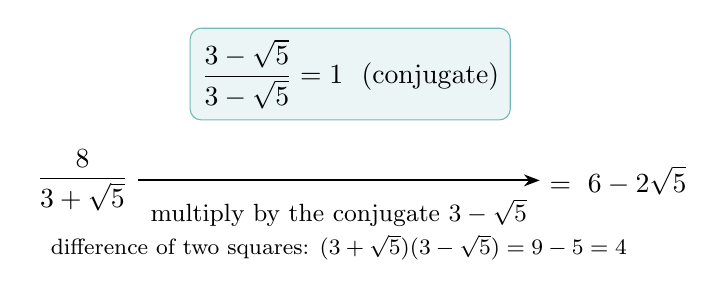
\begin{tikzpicture}[>={Stealth[length=2mm]}]
\node[draw=teal!55,rounded corners,fill=teal!8,inner sep=4pt] (rule) at (3.4,1.35) {$\displaystyle \frac{3-\sqrt5}{3-\sqrt5}=1$ \ (conjugate)};
\node (L) at (0,0) {$\displaystyle \frac{8}{3+\sqrt5}$};
\node (R) at (6.8,0) {$\displaystyle =\ 6-2\sqrt5$};
\draw[->,thick] (L) -- (R) node[midway,below=3pt,font=\small,align=center]{multiply by the conjugate $3-\sqrt5$\\[1pt]\footnotesize difference of two squares: $(3+\sqrt5)(3-\sqrt5)=9-5=4$};
\end{tikzpicture}
}
\end{center}
\small Multiply by the conjugate over itself. The denominator is then a difference of two squares, $(A+B)(A-B)=A^{2}-B^{2}$, so every surd cancels and the denominator becomes rational.\normalsize

\medskip\hrule

\section*{Rationalising the Denominator 25\quad\small\texttt{(a6-025)}}
\addcontentsline{toc}{section}{Rationalising the Denominator 25 (a6-025)}
\textit{Difficulty: Foundation \quad\textbar\quad Marks: 3}

\question{Express in the form \( a + b\sqrt{k} \) where \( a \), \( b \) and \( k \) are integers: \( \frac{25}{6 - \sqrt{11}} \)}

\textbf{Worked solution.}

\textit{Step 1: Multiply the top and bottom by the conjugate \( 6 + \sqrt{11} \).}
\[\begin{gathered}
\frac{25(6 + \sqrt{11})}{(6 - \sqrt{11})(6 + \sqrt{11})}
\end{gathered}\]
Switch the sign in the conjugate.

\textit{Step 2: Expand the denominator.}
\[\begin{gathered}
\frac{25(6 + \sqrt{11})}{36 - 11} = \frac{25(6 + \sqrt{11})}{25}
\end{gathered}\]
\( 6^2 - (\sqrt{11})^2 = 36 - 11 = 25 \).

\textit{Step 3: Cancel the common factor of 25.}
\[\begin{gathered}
6 + \sqrt{11}
\end{gathered}\]
The numerator and denominator both contain 25, which cancel to give \( a = 6 \), \( b = 1 \), \( k = 11 \).

\begin{answerbox}
\textbf{Final answer:}\quad \(\displaystyle 6 + \sqrt{11}\)
\end{answerbox}
\textbf{Diagram.}

\begin{center}
\resizebox{\ifdim\width>\linewidth \linewidth\else \width\fi}{!}{%
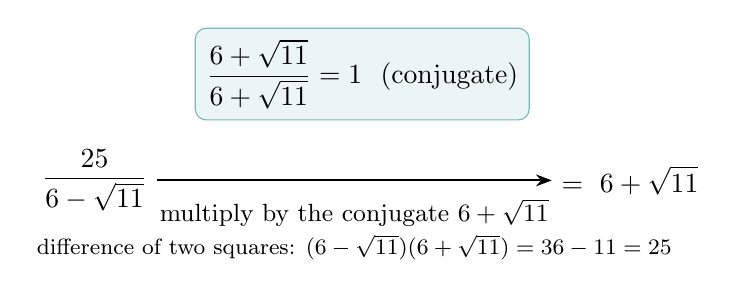
\begin{tikzpicture}[>={Stealth[length=2mm]}]
\node[draw=teal!55,rounded corners,fill=teal!8,inner sep=4pt] (rule) at (3.4,1.35) {$\displaystyle \frac{6+\sqrt{11}}{6+\sqrt{11}}=1$ \ (conjugate)};
\node (L) at (0,0) {$\displaystyle \frac{25}{6-\sqrt{11}}$};
\node (R) at (6.8,0) {$\displaystyle =\ 6+\sqrt{11}$};
\draw[->,thick] (L) -- (R) node[midway,below=3pt,font=\small,align=center]{multiply by the conjugate $6+\sqrt{11}$\\[1pt]\footnotesize difference of two squares: $(6-\sqrt{11})(6+\sqrt{11})=36-11=25$};
\end{tikzpicture}
}
\end{center}
\small Multiply by the conjugate over itself. The denominator is then a difference of two squares, $(A+B)(A-B)=A^{2}-B^{2}$, so every surd cancels and the denominator becomes rational.\normalsize

\medskip\hrule

\section*{Rationalising the Denominator 26\quad\small\texttt{(a6-026)}}
\addcontentsline{toc}{section}{Rationalising the Denominator 26 (a6-026)}
\textit{Difficulty: Foundation \quad\textbar\quad Marks: 4}

\question{Express in the form \( p + q\sqrt{r} \) where \( r \) is an integer, and \( p \) and \( q \) are integers or fractions: \( \frac{\sqrt{3} + 1}{\sqrt{3} - 1} \)}

\textbf{Worked solution.}

\textit{Step 1: Multiply the top and bottom by the conjugate \( \sqrt{3} + 1 \).}
\[\begin{gathered}
\frac{(\sqrt{3} + 1)(\sqrt{3} + 1)}{(\sqrt{3} - 1)(\sqrt{3} + 1)}
\end{gathered}\]
The conjugate of \( \sqrt{3} - 1 \) is \( \sqrt{3} + 1 \).

\textit{Step 2: Expand the numerator using \( (a+b)^2 = a^2 + 2ab + b^2 \).}
\[\begin{gathered}
\frac{3 + 2\sqrt{3} + 1}{3 - 1} = \frac{4 + 2\sqrt{3}}{2}
\end{gathered}\]
Numerator: \( (\sqrt{3})^2 + 2\sqrt{3} + 1 = 4 + 2\sqrt{3} \). Denominator: \( 3 - 1 = 2 \).

\textit{Step 3: Simplify by dividing each term by 2.}
\[\begin{gathered}
2 + \sqrt{3}
\end{gathered}\]
\( \frac{4}{2} = 2 \) and \( \frac{2\sqrt{3}}{2} = \sqrt{3} \).

\begin{answerbox}
\textbf{Final answer:}\quad \(\displaystyle 2 + \sqrt{3}\)
\end{answerbox}
\textbf{Diagram.}

\begin{center}
\resizebox{\ifdim\width>\linewidth \linewidth\else \width\fi}{!}{%
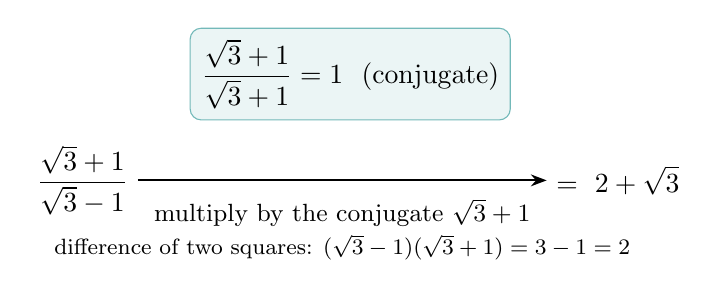
\begin{tikzpicture}[>={Stealth[length=2mm]}]
\node[draw=teal!55,rounded corners,fill=teal!8,inner sep=4pt] (rule) at (3.4,1.35) {$\displaystyle \frac{\sqrt3+1}{\sqrt3+1}=1$ \ (conjugate)};
\node (L) at (0,0) {$\displaystyle \frac{\sqrt3+1}{\sqrt3-1}$};
\node (R) at (6.8,0) {$\displaystyle =\ 2+\sqrt3$};
\draw[->,thick] (L) -- (R) node[midway,below=3pt,font=\small,align=center]{multiply by the conjugate $\sqrt3+1$\\[1pt]\footnotesize difference of two squares: $(\sqrt3-1)(\sqrt3+1)=3-1=2$};
\end{tikzpicture}
}
\end{center}
\small Multiply by the conjugate over itself. The denominator is then a difference of two squares, $(A+B)(A-B)=A^{2}-B^{2}$, so every surd cancels and the denominator becomes rational.\normalsize

\medskip\hrule

\section*{Rationalising the Denominator 27\quad\small\texttt{(a6-027)}}
\addcontentsline{toc}{section}{Rationalising the Denominator 27 (a6-027)}
\textit{Difficulty: Foundation \quad\textbar\quad Marks: 4}

\question{Express in the form \( p + q\sqrt{r} \) where \( r \) is an integer, and \( p \) and \( q \) are integers or fractions: \( \frac{\sqrt{7} + 2}{\sqrt{7} - 3} \)}

\textbf{Worked solution.}

\textit{Step 1: Multiply the top and bottom by the conjugate \( \sqrt{7} + 3 \).}
\[\begin{gathered}
\frac{(\sqrt{7} + 2)(\sqrt{7} + 3)}{(\sqrt{7} - 3)(\sqrt{7} + 3)}
\end{gathered}\]
Switch the sign between the terms in the denominator.

\textit{Step 2: Expand the numerator using FOIL.}
\[\begin{gathered}
\frac{7 + 3\sqrt{7} + 2\sqrt{7} + 6}{7 - 9} = \frac{13 + 5\sqrt{7}}{-2}
\end{gathered}\]
Numerator: \( \sqrt{7} \times \sqrt{7} + 3\sqrt{7} + 2\sqrt{7} + 6 = 7 + 5\sqrt{7} + 6 = 13 + 5\sqrt{7} \). Denominator: \( 7 - 9 = -2 \).

\textit{Step 3: Split the fraction to get the required form.}
\[\begin{gathered}
-\frac{13}{2} - \frac{5}{2}\sqrt{7}
\end{gathered}\]
Divide each term in the numerator by \( -2 \).

\begin{answerbox}
\textbf{Final answer:}\quad \(\displaystyle -\frac{13}{2} - \frac{5}{2}\sqrt{7}\)
\end{answerbox}
\textbf{Diagram.}

\begin{center}
\resizebox{\ifdim\width>\linewidth \linewidth\else \width\fi}{!}{%
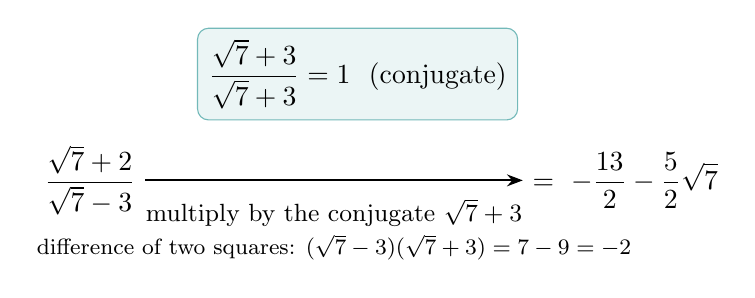
\begin{tikzpicture}[>={Stealth[length=2mm]}]
\node[draw=teal!55,rounded corners,fill=teal!8,inner sep=4pt] (rule) at (3.4,1.35) {$\displaystyle \frac{\sqrt7+3}{\sqrt7+3}=1$ \ (conjugate)};
\node (L) at (0,0) {$\displaystyle \frac{\sqrt7+2}{\sqrt7-3}$};
\node (R) at (6.8,0) {$\displaystyle =\ -\frac{13}{2}-\frac{5}{2}\sqrt7$};
\draw[->,thick] (L) -- (R) node[midway,below=3pt,font=\small,align=center]{multiply by the conjugate $\sqrt7+3$\\[1pt]\footnotesize difference of two squares: $(\sqrt7-3)(\sqrt7+3)=7-9=-2$};
\end{tikzpicture}
}
\end{center}
\small Multiply by the conjugate over itself. The denominator is then a difference of two squares, $(A+B)(A-B)=A^{2}-B^{2}$, so every surd cancels and the denominator becomes rational.\normalsize

\medskip\hrule

\section*{Rationalising the Denominator 28\quad\small\texttt{(a6-028)}}
\addcontentsline{toc}{section}{Rationalising the Denominator 28 (a6-028)}
\textit{Difficulty: Foundation \quad\textbar\quad Marks: 4}

\question{Express in the form \( p + q\sqrt{r} \) where \( r \) is an integer, and \( p \) and \( q \) are integers or fractions: \( \frac{5 - \sqrt{2}}{3 + \sqrt{2}} \)}

\textbf{Worked solution.}

\textit{Step 1: Multiply the top and bottom by the conjugate \( 3 - \sqrt{2} \).}
\[\begin{gathered}
\frac{(5 - \sqrt{2})(3 - \sqrt{2})}{(3 + \sqrt{2})(3 - \sqrt{2})}
\end{gathered}\]
Use the conjugate to eliminate the surd from the denominator.

\textit{Step 2: Expand the numerator and denominator.}
\[\begin{gathered}
\frac{15 - 5\sqrt{2} - 3\sqrt{2} + 2}{9 - 2} = \frac{17 - 8\sqrt{2}}{7}
\end{gathered}\]
Numerator: \( 15 - 5\sqrt{2} - 3\sqrt{2} + (\sqrt{2})^2 = 15 + 2 - 8\sqrt{2} = 17 - 8\sqrt{2} \). Denominator: \( 9 - 2 = 7 \).

\textit{Step 3: Split into the required form.}
\[\begin{gathered}
\frac{17}{7} - \frac{8}{7}\sqrt{2}
\end{gathered}\]
Divide each term by 7.

\begin{answerbox}
\textbf{Final answer:}\quad \(\displaystyle \frac{17}{7} - \frac{8}{7}\sqrt{2}\)
\end{answerbox}
\textbf{Diagram.}

\begin{center}
\resizebox{\ifdim\width>\linewidth \linewidth\else \width\fi}{!}{%
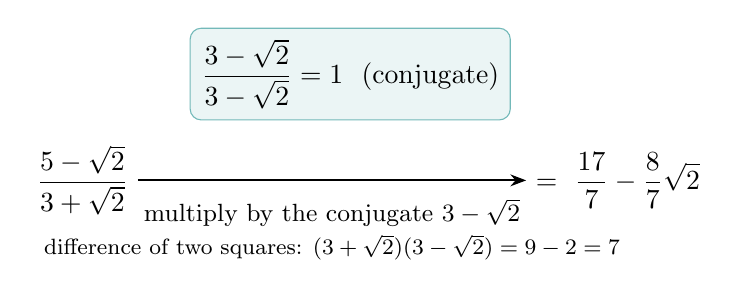
\begin{tikzpicture}[>={Stealth[length=2mm]}]
\node[draw=teal!55,rounded corners,fill=teal!8,inner sep=4pt] (rule) at (3.4,1.35) {$\displaystyle \frac{3-\sqrt2}{3-\sqrt2}=1$ \ (conjugate)};
\node (L) at (0,0) {$\displaystyle \frac{5-\sqrt2}{3+\sqrt2}$};
\node (R) at (6.8,0) {$\displaystyle =\ \frac{17}{7}-\frac{8}{7}\sqrt2$};
\draw[->,thick] (L) -- (R) node[midway,below=3pt,font=\small,align=center]{multiply by the conjugate $3-\sqrt2$\\[1pt]\footnotesize difference of two squares: $(3+\sqrt2)(3-\sqrt2)=9-2=7$};
\end{tikzpicture}
}
\end{center}
\small Multiply by the conjugate over itself. The denominator is then a difference of two squares, $(A+B)(A-B)=A^{2}-B^{2}$, so every surd cancels and the denominator becomes rational.\normalsize

\medskip\hrule

\section*{Rationalising the Denominator 29\quad\small\texttt{(a6-029)}}
\addcontentsline{toc}{section}{Rationalising the Denominator 29 (a6-029)}
\textit{Difficulty: Foundation \quad\textbar\quad Marks: 4}

\question{Express in the form \( p + q\sqrt{r} \) where \( r \) is an integer, and \( p \) and \( q \) are integers or fractions: \( \frac{2\sqrt{5} + 1}{3\sqrt{5} - 2} \)}

\textbf{Worked solution.}

\textit{Step 1: Multiply top and bottom by the conjugate \( 3\sqrt{5} + 2 \).}
\[\begin{gathered}
\frac{(2\sqrt{5} + 1)(3\sqrt{5} + 2)}{(3\sqrt{5} - 2)(3\sqrt{5} + 2)}
\end{gathered}\]
The conjugate flips the sign between the terms.

\textit{Step 2: Expand the numerator and denominator.}
\[\begin{gathered}
\frac{6 \times 5 + 4\sqrt{5} + 3\sqrt{5} + 2}{9 \times 5 - 4} = \frac{30 + 7\sqrt{5} + 2}{45 - 4} = \frac{32 + 7\sqrt{5}}{41}
\end{gathered}\]
Numerator: \( 2\sqrt{5} \times 3\sqrt{5} = 6 \times 5 = 30 \); cross terms: \( 4\sqrt{5} + 3\sqrt{5} = 7\sqrt{5} \); last: \( 1 \times 2 = 2 \). Denominator: \( (3\sqrt{5})^2 - 2^2 = 45 - 4 = 41 \).

\textit{Step 3: Split into the required form.}
\[\begin{gathered}
\frac{32}{41} + \frac{7}{41}\sqrt{5}
\end{gathered}\]
Divide each term by 41.

\begin{answerbox}
\textbf{Final answer:}\quad \(\displaystyle \frac{32}{41} + \frac{7}{41}\sqrt{5}\)
\end{answerbox}
\textbf{Diagram.}

\begin{center}
\resizebox{\ifdim\width>\linewidth \linewidth\else \width\fi}{!}{%
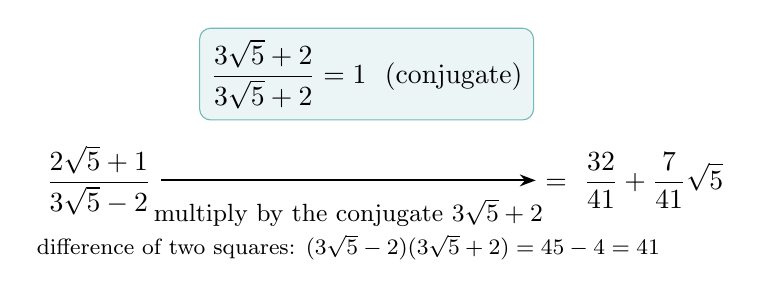
\begin{tikzpicture}[>={Stealth[length=2mm]}]
\node[draw=teal!55,rounded corners,fill=teal!8,inner sep=4pt] (rule) at (3.4,1.35) {$\displaystyle \frac{3\sqrt5+2}{3\sqrt5+2}=1$ \ (conjugate)};
\node (L) at (0,0) {$\displaystyle \frac{2\sqrt5+1}{3\sqrt5-2}$};
\node (R) at (6.8,0) {$\displaystyle =\ \frac{32}{41}+\frac{7}{41}\sqrt5$};
\draw[->,thick] (L) -- (R) node[midway,below=3pt,font=\small,align=center]{multiply by the conjugate $3\sqrt5+2$\\[1pt]\footnotesize difference of two squares: $(3\sqrt5-2)(3\sqrt5+2)=45-4=41$};
\end{tikzpicture}
}
\end{center}
\small Multiply by the conjugate over itself. The denominator is then a difference of two squares, $(A+B)(A-B)=A^{2}-B^{2}$, so every surd cancels and the denominator becomes rational.\normalsize

\medskip\hrule

\section*{Rationalising the Denominator 30\quad\small\texttt{(a6-030)}}
\addcontentsline{toc}{section}{Rationalising the Denominator 30 (a6-030)}
\textit{Difficulty: Foundation \quad\textbar\quad Marks: 4}

\question{Express in the form \( p + q\sqrt{r} \) where \( r \) is an integer, and \( p \) and \( q \) are integers or fractions: \( \frac{\sqrt{2} + 3}{2\sqrt{2} - 1} \)}

\textbf{Worked solution.}

\textit{Step 1: Multiply top and bottom by the conjugate \( 2\sqrt{2} + 1 \).}
\[\begin{gathered}
\frac{(\sqrt{2} + 3)(2\sqrt{2} + 1)}{(2\sqrt{2} - 1)(2\sqrt{2} + 1)}
\end{gathered}\]
Conjugate has opposite sign between the terms.

\textit{Step 2: Expand the numerator and denominator.}
\[\begin{gathered}
\frac{2 \times 2 + \sqrt{2} + 6\sqrt{2} + 3}{4 \times 2 - 1} = \frac{4 + 7\sqrt{2} + 3}{8 - 1} = \frac{7 + 7\sqrt{2}}{7}
\end{gathered}\]
Numerator: \( \sqrt{2} \times 2\sqrt{2} = 4 \); cross terms: \( \sqrt{2} + 6\sqrt{2} = 7\sqrt{2} \); last: 3. Denominator: \( (2\sqrt{2})^2 - 1 = 8 - 1 = 7 \).

\textit{Step 3: Simplify.}
\[\begin{gathered}
1 + \sqrt{2}
\end{gathered}\]
Divide each term by 7.

\begin{answerbox}
\textbf{Final answer:}\quad \(\displaystyle 1 + \sqrt{2}\)
\end{answerbox}
\textbf{Diagram.}

\begin{center}
\resizebox{\ifdim\width>\linewidth \linewidth\else \width\fi}{!}{%
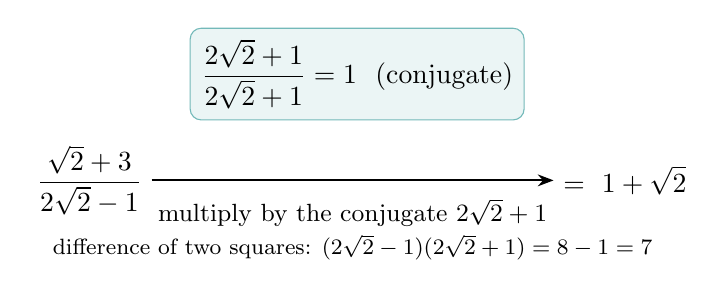
\begin{tikzpicture}[>={Stealth[length=2mm]}]
\node[draw=teal!55,rounded corners,fill=teal!8,inner sep=4pt] (rule) at (3.4,1.35) {$\displaystyle \frac{2\sqrt2+1}{2\sqrt2+1}=1$ \ (conjugate)};
\node (L) at (0,0) {$\displaystyle \frac{\sqrt2+3}{2\sqrt2-1}$};
\node (R) at (6.8,0) {$\displaystyle =\ 1+\sqrt2$};
\draw[->,thick] (L) -- (R) node[midway,below=3pt,font=\small,align=center]{multiply by the conjugate $2\sqrt2+1$\\[1pt]\footnotesize difference of two squares: $(2\sqrt2-1)(2\sqrt2+1)=8-1=7$};
\end{tikzpicture}
}
\end{center}
\small Multiply by the conjugate over itself. The denominator is then a difference of two squares, $(A+B)(A-B)=A^{2}-B^{2}$, so every surd cancels and the denominator becomes rational.\normalsize

\medskip\hrule

\section*{Rationalising the Denominator 31\quad\small\texttt{(a6-031)}}
\addcontentsline{toc}{section}{Rationalising the Denominator 31 (a6-031)}
\textit{Difficulty: Foundation \quad\textbar\quad Marks: 4}

\question{Express in the form \( p + q\sqrt{r} \) where \( r \) is an integer, and \( p \) and \( q \) are integers or fractions: \( \frac{4 - \sqrt{3}}{2 + \sqrt{3}} \)}

\textbf{Worked solution.}

\textit{Step 1: Multiply top and bottom by the conjugate \( 2 - \sqrt{3} \).}
\[\begin{gathered}
\frac{(4 - \sqrt{3})(2 - \sqrt{3})}{(2 + \sqrt{3})(2 - \sqrt{3})}
\end{gathered}\]
Flip the sign in the denominator to form the conjugate.

\textit{Step 2: Expand the numerator and denominator.}
\[\begin{gathered}
\frac{8 - 4\sqrt{3} - 2\sqrt{3} + 3}{4 - 3} = \frac{11 - 6\sqrt{3}}{1}
\end{gathered}\]
Numerator: \( 8 - 4\sqrt{3} - 2\sqrt{3} + (\sqrt{3})^2 = 8 + 3 - 6\sqrt{3} = 11 - 6\sqrt{3} \). Denominator: \( 4 - 3 = 1 \).

\textit{Step 3: Write final answer.}
\[\begin{gathered}
11 - 6\sqrt{3}
\end{gathered}\]
Dividing by 1 leaves the numerator unchanged.

\begin{answerbox}
\textbf{Final answer:}\quad \(\displaystyle 11 - 6\sqrt{3}\)
\end{answerbox}
\textbf{Diagram.}

\begin{center}
\resizebox{\ifdim\width>\linewidth \linewidth\else \width\fi}{!}{%
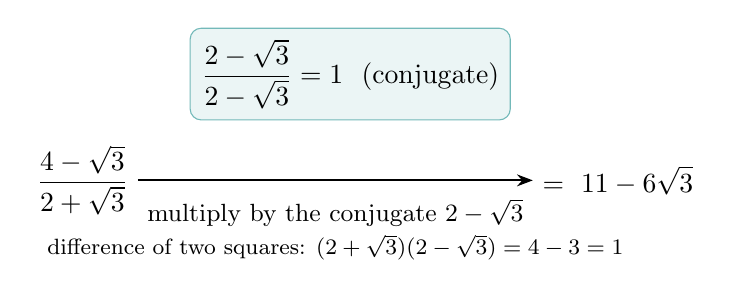
\begin{tikzpicture}[>={Stealth[length=2mm]}]
\node[draw=teal!55,rounded corners,fill=teal!8,inner sep=4pt] (rule) at (3.4,1.35) {$\displaystyle \frac{2-\sqrt3}{2-\sqrt3}=1$ \ (conjugate)};
\node (L) at (0,0) {$\displaystyle \frac{4-\sqrt3}{2+\sqrt3}$};
\node (R) at (6.8,0) {$\displaystyle =\ 11-6\sqrt3$};
\draw[->,thick] (L) -- (R) node[midway,below=3pt,font=\small,align=center]{multiply by the conjugate $2-\sqrt3$\\[1pt]\footnotesize difference of two squares: $(2+\sqrt3)(2-\sqrt3)=4-3=1$};
\end{tikzpicture}
}
\end{center}
\small Multiply by the conjugate over itself. The denominator is then a difference of two squares, $(A+B)(A-B)=A^{2}-B^{2}$, so every surd cancels and the denominator becomes rational.\normalsize

\medskip\hrule

\section*{Rationalising the Denominator 32\quad\small\texttt{(a6-032)}}
\addcontentsline{toc}{section}{Rationalising the Denominator 32 (a6-032)}
\textit{Difficulty: Foundation \quad\textbar\quad Marks: 4}

\question{Express in the form \( k(\sqrt{x} \pm \sqrt{y}) \), where \( x \) and \( y \) are integers and \( k \) is an integer or fraction: \( \frac{6}{\sqrt{5} - \sqrt{2}} \)}

\textbf{Worked solution.}

\textit{Step 1: Multiply top and bottom by the conjugate \( \sqrt{5} + \sqrt{2} \).}
\[\begin{gathered}
\frac{6(\sqrt{5} + \sqrt{2})}{(\sqrt{5} - \sqrt{2})(\sqrt{5} + \sqrt{2})}
\end{gathered}\]
The conjugate of \( \sqrt{5} - \sqrt{2} \) is \( \sqrt{5} + \sqrt{2} \).

\textit{Step 2: Expand the denominator.}
\[\begin{gathered}
\frac{6(\sqrt{5} + \sqrt{2})}{5 - 2} = \frac{6(\sqrt{5} + \sqrt{2})}{3}
\end{gathered}\]
\( (\sqrt{5})^2 - (\sqrt{2})^2 = 5 - 2 = 3 \).

\textit{Step 3: Simplify by dividing by 3.}
\[\begin{gathered}
2(\sqrt{5} + \sqrt{2})
\end{gathered}\]
\( \frac{6}{3} = 2 \). So \( k = 2 \), \( x = 5 \), \( y = 2 \).

\begin{answerbox}
\textbf{Final answer:}\quad \(\displaystyle 2(\sqrt{5} + \sqrt{2})\)
\end{answerbox}
\textbf{Diagram.}

\begin{center}
\resizebox{\ifdim\width>\linewidth \linewidth\else \width\fi}{!}{%
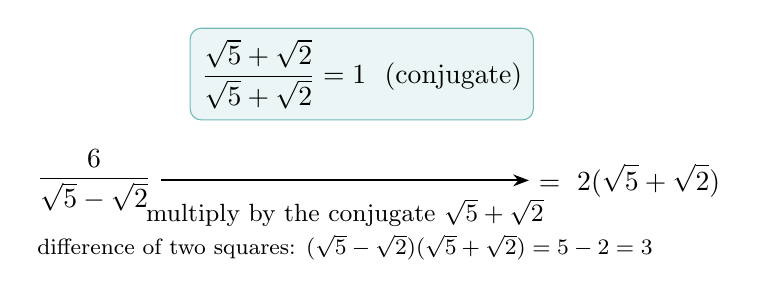
\begin{tikzpicture}[>={Stealth[length=2mm]}]
\node[draw=teal!55,rounded corners,fill=teal!8,inner sep=4pt] (rule) at (3.4,1.35) {$\displaystyle \frac{\sqrt5+\sqrt2}{\sqrt5+\sqrt2}=1$ \ (conjugate)};
\node (L) at (0,0) {$\displaystyle \frac{6}{\sqrt5-\sqrt2}$};
\node (R) at (6.8,0) {$\displaystyle =\ 2(\sqrt5+\sqrt2)$};
\draw[->,thick] (L) -- (R) node[midway,below=3pt,font=\small,align=center]{multiply by the conjugate $\sqrt5+\sqrt2$\\[1pt]\footnotesize difference of two squares: $(\sqrt5-\sqrt2)(\sqrt5+\sqrt2)=5-2=3$};
\end{tikzpicture}
}
\end{center}
\small Multiply by the conjugate over itself. The denominator is then a difference of two squares, $(A+B)(A-B)=A^{2}-B^{2}$, so every surd cancels and the denominator becomes rational.\normalsize

\medskip\hrule

\section*{Rationalising the Denominator 33\quad\small\texttt{(a6-033)}}
\addcontentsline{toc}{section}{Rationalising the Denominator 33 (a6-033)}
\textit{Difficulty: Foundation \quad\textbar\quad Marks: 4}

\question{Express in the form \( k(\sqrt{x} \pm \sqrt{y}) \), where \( x \) and \( y \) are integers and \( k \) is an integer or fraction: \( \frac{10}{\sqrt{7} + \sqrt{2}} \)}

\textbf{Worked solution.}

\textit{Step 1: Multiply top and bottom by the conjugate \( \sqrt{7} - \sqrt{2} \).}
\[\begin{gathered}
\frac{10(\sqrt{7} - \sqrt{2})}{(\sqrt{7} + \sqrt{2})(\sqrt{7} - \sqrt{2})}
\end{gathered}\]
Switch the sign between the surds.

\textit{Step 2: Expand the denominator.}
\[\begin{gathered}
\frac{10(\sqrt{7} - \sqrt{2})}{7 - 2} = \frac{10(\sqrt{7} - \sqrt{2})}{5}
\end{gathered}\]
\( 7 - 2 = 5 \).

\textit{Step 3: Simplify.}
\[\begin{gathered}
2(\sqrt{7} - \sqrt{2})
\end{gathered}\]
\( \frac{10}{5} = 2 \).

\begin{answerbox}
\textbf{Final answer:}\quad \(\displaystyle 2(\sqrt{7} - \sqrt{2})\)
\end{answerbox}
\textbf{Diagram.}

\begin{center}
\resizebox{\ifdim\width>\linewidth \linewidth\else \width\fi}{!}{%
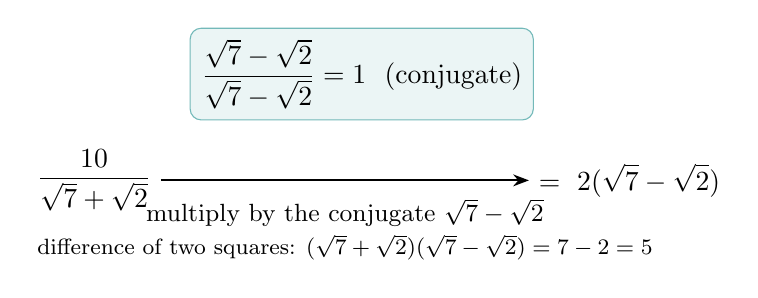
\begin{tikzpicture}[>={Stealth[length=2mm]}]
\node[draw=teal!55,rounded corners,fill=teal!8,inner sep=4pt] (rule) at (3.4,1.35) {$\displaystyle \frac{\sqrt7-\sqrt2}{\sqrt7-\sqrt2}=1$ \ (conjugate)};
\node (L) at (0,0) {$\displaystyle \frac{10}{\sqrt7+\sqrt2}$};
\node (R) at (6.8,0) {$\displaystyle =\ 2(\sqrt7-\sqrt2)$};
\draw[->,thick] (L) -- (R) node[midway,below=3pt,font=\small,align=center]{multiply by the conjugate $\sqrt7-\sqrt2$\\[1pt]\footnotesize difference of two squares: $(\sqrt7+\sqrt2)(\sqrt7-\sqrt2)=7-2=5$};
\end{tikzpicture}
}
\end{center}
\small Multiply by the conjugate over itself. The denominator is then a difference of two squares, $(A+B)(A-B)=A^{2}-B^{2}$, so every surd cancels and the denominator becomes rational.\normalsize

\medskip\hrule

\section*{Rationalising the Denominator 34\quad\small\texttt{(a6-034)}}
\addcontentsline{toc}{section}{Rationalising the Denominator 34 (a6-034)}
\textit{Difficulty: Foundation \quad\textbar\quad Marks: 4}

\question{Express in the form \( k(\sqrt{x} \pm \sqrt{y}) \), where \( x \) and \( y \) are integers and \( k \) is an integer or fraction: \( \frac{3}{\sqrt{10} - \sqrt{7}} \)}

\textbf{Worked solution.}

\textit{Step 1: Multiply top and bottom by the conjugate \( \sqrt{10} + \sqrt{7} \).}
\[\begin{gathered}
\frac{3(\sqrt{10} + \sqrt{7})}{(\sqrt{10} - \sqrt{7})(\sqrt{10} + \sqrt{7})}
\end{gathered}\]
Use the conjugate rule.

\textit{Step 2: Expand the denominator.}
\[\begin{gathered}
\frac{3(\sqrt{10} + \sqrt{7})}{10 - 7} = \frac{3(\sqrt{10} + \sqrt{7})}{3}
\end{gathered}\]
\( 10 - 7 = 3 \).

\textit{Step 3: Cancel.}
\[\begin{gathered}
\sqrt{10} + \sqrt{7}
\end{gathered}\]
The 3s cancel, so \( k = 1 \), \( x = 10 \), \( y = 7 \).

\begin{answerbox}
\textbf{Final answer:}\quad \(\displaystyle \sqrt{10} + \sqrt{7}\)
\end{answerbox}
\textbf{Diagram.}

\begin{center}
\resizebox{\ifdim\width>\linewidth \linewidth\else \width\fi}{!}{%
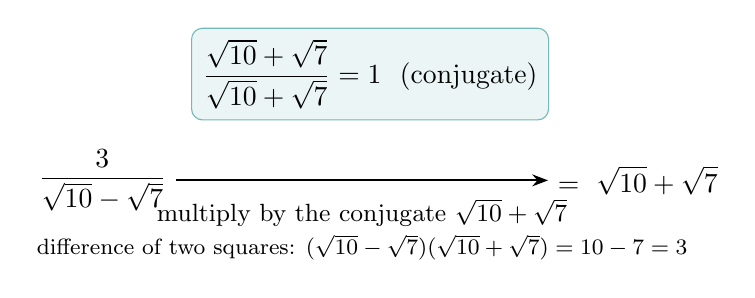
\begin{tikzpicture}[>={Stealth[length=2mm]}]
\node[draw=teal!55,rounded corners,fill=teal!8,inner sep=4pt] (rule) at (3.4,1.35) {$\displaystyle \frac{\sqrt{10}+\sqrt7}{\sqrt{10}+\sqrt7}=1$ \ (conjugate)};
\node (L) at (0,0) {$\displaystyle \frac{3}{\sqrt{10}-\sqrt7}$};
\node (R) at (6.8,0) {$\displaystyle =\ \sqrt{10}+\sqrt7$};
\draw[->,thick] (L) -- (R) node[midway,below=3pt,font=\small,align=center]{multiply by the conjugate $\sqrt{10}+\sqrt7$\\[1pt]\footnotesize difference of two squares: $(\sqrt{10}-\sqrt7)(\sqrt{10}+\sqrt7)=10-7=3$};
\end{tikzpicture}
}
\end{center}
\small Multiply by the conjugate over itself. The denominator is then a difference of two squares, $(A+B)(A-B)=A^{2}-B^{2}$, so every surd cancels and the denominator becomes rational.\normalsize

\medskip\hrule

\section*{Rationalising the Denominator 35\quad\small\texttt{(a6-035)}}
\addcontentsline{toc}{section}{Rationalising the Denominator 35 (a6-035)}
\textit{Difficulty: Foundation \quad\textbar\quad Marks: 4}

\question{Express in the form \( k(\sqrt{x} \pm \sqrt{y}) \), where \( x \) and \( y \) are integers and \( k \) is an integer or fraction: \( \frac{8}{\sqrt{11} + \sqrt{3}} \)}

\textbf{Worked solution.}

\textit{Step 1: Multiply top and bottom by the conjugate \( \sqrt{11} - \sqrt{3} \).}
\[\begin{gathered}
\frac{8(\sqrt{11} - \sqrt{3})}{(\sqrt{11} + \sqrt{3})(\sqrt{11} - \sqrt{3})}
\end{gathered}\]
Flip the sign between the surds.

\textit{Step 2: Expand the denominator.}
\[\begin{gathered}
\frac{8(\sqrt{11} - \sqrt{3})}{11 - 3} = \frac{8(\sqrt{11} - \sqrt{3})}{8}
\end{gathered}\]
\( 11 - 3 = 8 \).

\textit{Step 3: Cancel.}
\[\begin{gathered}
\sqrt{11} - \sqrt{3}
\end{gathered}\]
The 8s cancel.

\begin{answerbox}
\textbf{Final answer:}\quad \(\displaystyle \sqrt{11} - \sqrt{3}\)
\end{answerbox}
\textbf{Diagram.}

\begin{center}
\resizebox{\ifdim\width>\linewidth \linewidth\else \width\fi}{!}{%
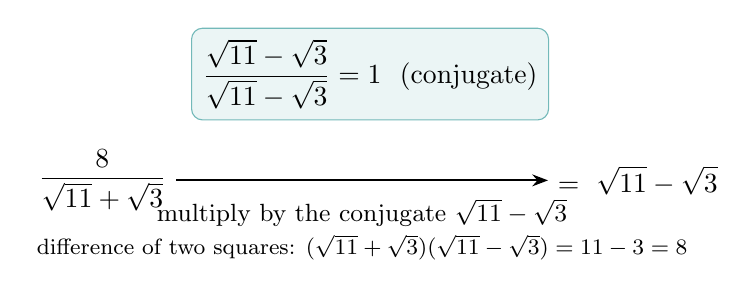
\begin{tikzpicture}[>={Stealth[length=2mm]}]
\node[draw=teal!55,rounded corners,fill=teal!8,inner sep=4pt] (rule) at (3.4,1.35) {$\displaystyle \frac{\sqrt{11}-\sqrt3}{\sqrt{11}-\sqrt3}=1$ \ (conjugate)};
\node (L) at (0,0) {$\displaystyle \frac{8}{\sqrt{11}+\sqrt3}$};
\node (R) at (6.8,0) {$\displaystyle =\ \sqrt{11}-\sqrt3$};
\draw[->,thick] (L) -- (R) node[midway,below=3pt,font=\small,align=center]{multiply by the conjugate $\sqrt{11}-\sqrt3$\\[1pt]\footnotesize difference of two squares: $(\sqrt{11}+\sqrt3)(\sqrt{11}-\sqrt3)=11-3=8$};
\end{tikzpicture}
}
\end{center}
\small Multiply by the conjugate over itself. The denominator is then a difference of two squares, $(A+B)(A-B)=A^{2}-B^{2}$, so every surd cancels and the denominator becomes rational.\normalsize

\medskip\hrule

\section*{Rationalising the Denominator 36\quad\small\texttt{(a6-036)}}
\addcontentsline{toc}{section}{Rationalising the Denominator 36 (a6-036)}
\textit{Difficulty: Foundation \quad\textbar\quad Marks: 2}

\question{Rationalise and simplify: \( \frac{7}{\sqrt{11}} \)}

\textbf{Worked solution.}

\textit{Multiply the top and bottom by \( \sqrt{11} \).}
\[\begin{gathered}
\frac{7\sqrt{11}}{11}
\end{gathered}\]
\( \sqrt{11} \times \sqrt{11} = 11 \).

\begin{answerbox}
\textbf{Final answer:}\quad \(\displaystyle \frac{7\sqrt{11}}{11}\)
\end{answerbox}
\textbf{Diagram.}

\begin{center}
\resizebox{\ifdim\width>\linewidth \linewidth\else \width\fi}{!}{%
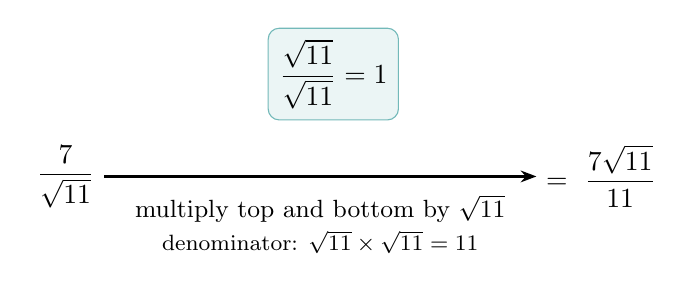
\begin{tikzpicture}[>={Stealth[length=2mm]}]
\node[draw=teal!55,rounded corners,fill=teal!8,inner sep=4pt] (rule) at (3.4,1.3) {$\displaystyle \frac{\sqrt{11}}{\sqrt{11}}=1$};
\node (L) at (0,0) {$\displaystyle \frac{7}{\sqrt{11}}$};
\node (R) at (6.8,0) {$\displaystyle =\ \frac{7\sqrt{11}}{11}$};
\draw[->,thick] (L) -- (R) node[midway,below=3pt,font=\small,align=center]{multiply top and bottom by $\sqrt{11}$\\[1pt]\footnotesize denominator: $\sqrt{11}\times\sqrt{11}=11$};
\end{tikzpicture}
}
\end{center}
\small Multiply by $\frac{\sqrt{a}}{\sqrt{a}}=1$: this leaves the value unchanged but clears the surd from the denominator.\normalsize

\medskip\hrule

\section*{Rationalising the Denominator 37\quad\small\texttt{(a6-037)}}
\addcontentsline{toc}{section}{Rationalising the Denominator 37 (a6-037)}
\textit{Difficulty: Foundation \quad\textbar\quad Marks: 3}

\question{Rationalise and simplify: \( \frac{\sqrt{5}}{\sqrt{12}} \)}

\textbf{Worked solution.}

\textit{Step 1: Simplify \( \sqrt{12} \).}
\[\begin{gathered}
\frac{\sqrt{5}}{\sqrt{12}} = \frac{\sqrt{5}}{2\sqrt{3}}
\end{gathered}\]
\( \sqrt{12} = 2\sqrt{3} \).

\textit{Step 2: Multiply the top and bottom by \( \sqrt{3} \).}
\[\begin{gathered}
\frac{\sqrt{5} \times \sqrt{3}}{2\sqrt{3} \times \sqrt{3}} = \frac{\sqrt{15}}{6}
\end{gathered}\]
\( \sqrt{5} \times \sqrt{3} = \sqrt{15} \) and \( 2\sqrt{3} \times \sqrt{3} = 2 \times 3 = 6 \).

\begin{answerbox}
\textbf{Final answer:}\quad \(\displaystyle \frac{\sqrt{15}}{6}\)
\end{answerbox}
\textbf{Diagram.}

\begin{center}
\resizebox{\ifdim\width>\linewidth \linewidth\else \width\fi}{!}{%
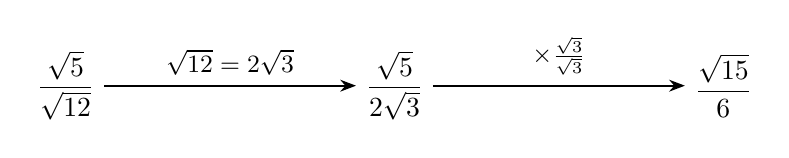
\begin{tikzpicture}[>={Stealth[length=2mm]},node distance=1.5cm and 3.2cm]
\node (s0) {$\displaystyle \frac{\sqrt5}{\sqrt{12}}$};
\node (s1) [right=of s0] {$\displaystyle \frac{\sqrt5}{2\sqrt3}$};
\node (s2) [right=of s1] {$\displaystyle \frac{\sqrt{15}}{6}$};
\draw[->,thick] (s0) -- (s1) node[midway,above,font=\small]{$\sqrt{12}=2\sqrt3$};
\draw[->,thick] (s1) -- (s2) node[midway,above,font=\small]{$\times\tfrac{\sqrt3}{\sqrt3}$};
\end{tikzpicture}
}
\end{center}
\small Solution flow: each arrow applies one step.\normalsize

\medskip\hrule

\section*{Rationalising the Denominator 38\quad\small\texttt{(a6-038)}}
\addcontentsline{toc}{section}{Rationalising the Denominator 38 (a6-038)}
\textit{Difficulty: Foundation \quad\textbar\quad Marks: 4}

\question{Simplify, giving your answer in the form \( p\sqrt{q} \) where \( p \) and \( q \) are integers: \( \frac{\sqrt{200}}{5} + \frac{30}{\sqrt{50}} \)}

\textbf{Worked solution.}

\textit{Step 1: Simplify the first fraction.}
\[\begin{gathered}
\frac{\sqrt{200}}{5} = \frac{10\sqrt{2}}{5} = 2\sqrt{2}
\end{gathered}\]
\( \sqrt{200} = 10\sqrt{2} \), then divide by 5.

\textit{Step 2: Rationalise and simplify the second fraction.}
\[\begin{gathered}
\frac{30}{\sqrt{50}} = \frac{30}{5\sqrt{2}} = \frac{6}{\sqrt{2}} = \frac{6\sqrt{2}}{2} = 3\sqrt{2}
\end{gathered}\]
\( \sqrt{50} = 5\sqrt{2} \), simplify to \( \frac{6}{\sqrt{2}} \), then rationalise.

\textit{Step 3: Add the like surds.}
\[\begin{gathered}
2\sqrt{2} + 3\sqrt{2} = 5\sqrt{2}
\end{gathered}\]
\( 2 + 3 = 5 \).

\begin{answerbox}
\textbf{Final answer:}\quad \(\displaystyle 5\sqrt{2}\)
\end{answerbox}
\textbf{Diagram.}

\begin{center}
\resizebox{\ifdim\width>\linewidth \linewidth\else \width\fi}{!}{%
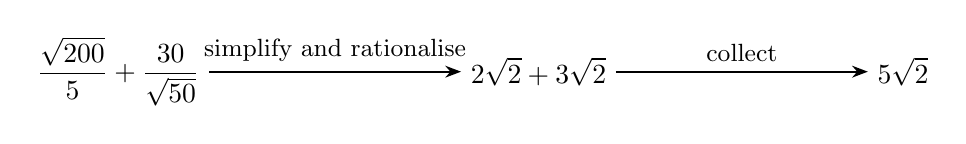
\begin{tikzpicture}[>={Stealth[length=2mm]},node distance=1.5cm and 3.2cm]
\node (s0) {$\displaystyle \frac{\sqrt{200}}{5}+\frac{30}{\sqrt{50}}$};
\node (s1) [right=of s0] {$\displaystyle 2\sqrt2+3\sqrt2$};
\node (s2) [right=of s1] {$\displaystyle 5\sqrt2$};
\draw[->,thick] (s0) -- (s1) node[midway,above,font=\small]{simplify and rationalise};
\draw[->,thick] (s1) -- (s2) node[midway,above,font=\small]{collect};
\end{tikzpicture}
}
\end{center}
\small Solution flow: each arrow applies one step.\normalsize

\medskip\hrule

\section*{Rationalising the Denominator 39\quad\small\texttt{(a6-039)}}
\addcontentsline{toc}{section}{Rationalising the Denominator 39 (a6-039)}
\textit{Difficulty: Foundation \quad\textbar\quad Marks: 2}

\question{Rationalise the denominator: \( \frac{2}{3\sqrt{5}} \)}

\textbf{Worked solution.}

\textit{Multiply the top and bottom by \( \sqrt{5} \).}
\[\begin{gathered}
\frac{2\sqrt{5}}{3 \times 5} = \frac{2\sqrt{5}}{15}
\end{gathered}\]
\( 3\sqrt{5} \times \sqrt{5} = 3 \times 5 = 15 \).

\begin{answerbox}
\textbf{Final answer:}\quad \(\displaystyle \frac{2\sqrt{5}}{15}\)
\end{answerbox}
\textbf{Diagram.}

\begin{center}
\resizebox{\ifdim\width>\linewidth \linewidth\else \width\fi}{!}{%
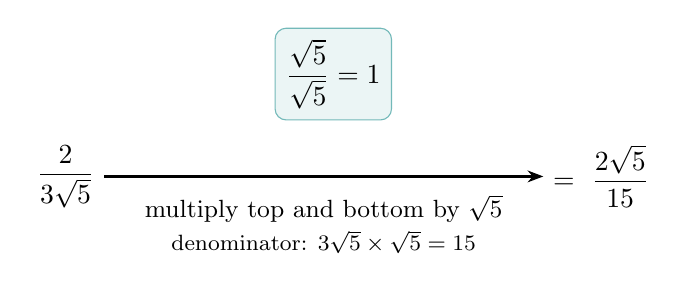
\begin{tikzpicture}[>={Stealth[length=2mm]}]
\node[draw=teal!55,rounded corners,fill=teal!8,inner sep=4pt] (rule) at (3.4,1.3) {$\displaystyle \frac{\sqrt5}{\sqrt5}=1$};
\node (L) at (0,0) {$\displaystyle \frac{2}{3\sqrt5}$};
\node (R) at (6.8,0) {$\displaystyle =\ \frac{2\sqrt5}{15}$};
\draw[->,thick] (L) -- (R) node[midway,below=3pt,font=\small,align=center]{multiply top and bottom by $\sqrt5$\\[1pt]\footnotesize denominator: $3\sqrt5\times\sqrt5=15$};
\end{tikzpicture}
}
\end{center}
\small Multiply by $\frac{\sqrt{a}}{\sqrt{a}}=1$: this leaves the value unchanged but clears the surd from the denominator.\normalsize

\medskip\hrule

\section*{Rationalising the Denominator 40\quad\small\texttt{(a6-040)}}
\addcontentsline{toc}{section}{Rationalising the Denominator 40 (a6-040)}
\textit{Difficulty: Foundation \quad\textbar\quad Marks: 2}

\question{Rationalise the denominator and simplify: \( \frac{\sqrt{45}}{\sqrt{5}} \)}

\textbf{Worked solution.}

\textit{Step 1: Combine the surds under a single root.}
\[\begin{gathered}
\sqrt{\frac{45}{5}} = \sqrt{9}
\end{gathered}\]
Use \( \frac{\sqrt{a}}{\sqrt{b}} = \sqrt{\frac{a}{b}} \).

\textit{Step 2: Evaluate.}
\[\begin{gathered}
3
\end{gathered}\]
\( \sqrt{9} = 3 \).

\begin{answerbox}
\textbf{Final answer:}\quad \(\displaystyle 3\)
\end{answerbox}
\textbf{Diagram.}

\begin{center}
\resizebox{\ifdim\width>\linewidth \linewidth\else \width\fi}{!}{%
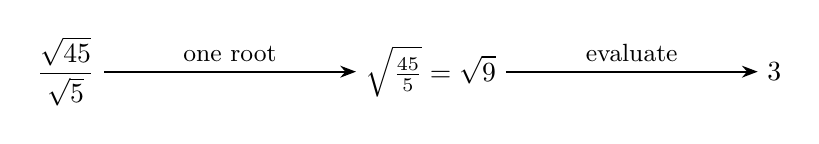
\begin{tikzpicture}[>={Stealth[length=2mm]},node distance=1.5cm and 3.2cm]
\node (s0) {$\displaystyle \frac{\sqrt{45}}{\sqrt5}$};
\node (s1) [right=of s0] {$\displaystyle \sqrt{\tfrac{45}{5}}=\sqrt9$};
\node (s2) [right=of s1] {$\displaystyle 3$};
\draw[->,thick] (s0) -- (s1) node[midway,above,font=\small]{one root};
\draw[->,thick] (s1) -- (s2) node[midway,above,font=\small]{evaluate};
\end{tikzpicture}
}
\end{center}
\small Solution flow: each arrow applies one step.\normalsize

\medskip\hrule

\section*{Rationalising the Denominator 41\quad\small\texttt{(a6-041)}}
\addcontentsline{toc}{section}{Rationalising the Denominator 41 (a6-041)}
\textit{Difficulty: Foundation \quad\textbar\quad Marks: 3}

\question{Express in the form \( a + b\sqrt{k} \) where \( a \), \( b \) and \( k \) are integers: \( \frac{6}{4 - \sqrt{10}} \)}

\textbf{Worked solution.}

\textit{Step 1: Multiply top and bottom by the conjugate \( 4 + \sqrt{10} \).}
\[\begin{gathered}
\frac{6(4 + \sqrt{10})}{(4 - \sqrt{10})(4 + \sqrt{10})}
\end{gathered}\]
Flip the sign to get the conjugate.

\textit{Step 2: Expand the denominator.}
\[\begin{gathered}
\frac{6(4 + \sqrt{10})}{16 - 10} = \frac{6(4 + \sqrt{10})}{6}
\end{gathered}\]
\( 4^2 - 10 = 16 - 10 = 6 \).

\textit{Step 3: Cancel.}
\[\begin{gathered}
4 + \sqrt{10}
\end{gathered}\]
The 6s cancel exactly.

\begin{answerbox}
\textbf{Final answer:}\quad \(\displaystyle 4 + \sqrt{10}\)
\end{answerbox}
\textbf{Diagram.}

\begin{center}
\resizebox{\ifdim\width>\linewidth \linewidth\else \width\fi}{!}{%
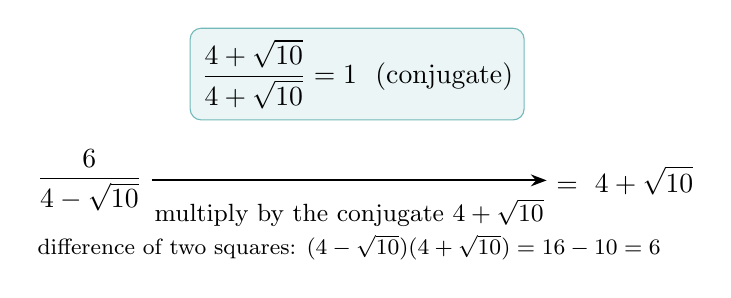
\begin{tikzpicture}[>={Stealth[length=2mm]}]
\node[draw=teal!55,rounded corners,fill=teal!8,inner sep=4pt] (rule) at (3.4,1.35) {$\displaystyle \frac{4+\sqrt{10}}{4+\sqrt{10}}=1$ \ (conjugate)};
\node (L) at (0,0) {$\displaystyle \frac{6}{4-\sqrt{10}}$};
\node (R) at (6.8,0) {$\displaystyle =\ 4+\sqrt{10}$};
\draw[->,thick] (L) -- (R) node[midway,below=3pt,font=\small,align=center]{multiply by the conjugate $4+\sqrt{10}$\\[1pt]\footnotesize difference of two squares: $(4-\sqrt{10})(4+\sqrt{10})=16-10=6$};
\end{tikzpicture}
}
\end{center}
\small Multiply by the conjugate over itself. The denominator is then a difference of two squares, $(A+B)(A-B)=A^{2}-B^{2}$, so every surd cancels and the denominator becomes rational.\normalsize

\medskip\hrule

\section*{Rationalising the Denominator 42\quad\small\texttt{(a6-042)}}
\addcontentsline{toc}{section}{Rationalising the Denominator 42 (a6-042)}
\textit{Difficulty: Foundation \quad\textbar\quad Marks: 3}

\question{Express in the form \( a + b\sqrt{k} \) where \( a \), \( b \) and \( k \) are integers: \( \frac{32}{7 - \sqrt{17}} \)}

\textbf{Worked solution.}

\textit{Step 1: Multiply top and bottom by the conjugate \( 7 + \sqrt{17} \).}
\[\begin{gathered}
\frac{32(7 + \sqrt{17})}{(7 - \sqrt{17})(7 + \sqrt{17})}
\end{gathered}\]
Use the conjugate to rationalise.

\textit{Step 2: Expand the denominator.}
\[\begin{gathered}
\frac{32(7 + \sqrt{17})}{49 - 17} = \frac{32(7 + \sqrt{17})}{32}
\end{gathered}\]
\( 49 - 17 = 32 \).

\textit{Step 3: Cancel the common factor of 32.}
\[\begin{gathered}
7 + \sqrt{17}
\end{gathered}\]
Numerator and denominator both contain 32, giving \( a = 7 \), \( b = 1 \), \( k = 17 \).

\begin{answerbox}
\textbf{Final answer:}\quad \(\displaystyle 7 + \sqrt{17}\)
\end{answerbox}
\textbf{Diagram.}

\begin{center}
\resizebox{\ifdim\width>\linewidth \linewidth\else \width\fi}{!}{%
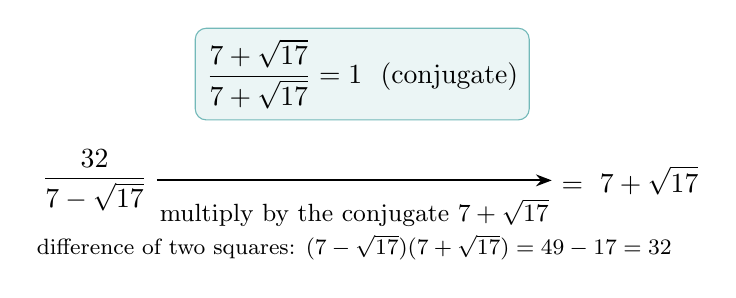
\begin{tikzpicture}[>={Stealth[length=2mm]}]
\node[draw=teal!55,rounded corners,fill=teal!8,inner sep=4pt] (rule) at (3.4,1.35) {$\displaystyle \frac{7+\sqrt{17}}{7+\sqrt{17}}=1$ \ (conjugate)};
\node (L) at (0,0) {$\displaystyle \frac{32}{7-\sqrt{17}}$};
\node (R) at (6.8,0) {$\displaystyle =\ 7+\sqrt{17}$};
\draw[->,thick] (L) -- (R) node[midway,below=3pt,font=\small,align=center]{multiply by the conjugate $7+\sqrt{17}$\\[1pt]\footnotesize difference of two squares: $(7-\sqrt{17})(7+\sqrt{17})=49-17=32$};
\end{tikzpicture}
}
\end{center}
\small Multiply by the conjugate over itself. The denominator is then a difference of two squares, $(A+B)(A-B)=A^{2}-B^{2}$, so every surd cancels and the denominator becomes rational.\normalsize

\medskip\hrule

\section*{Rationalising the Denominator 43\quad\small\texttt{(a6-043)}}
\addcontentsline{toc}{section}{Rationalising the Denominator 43 (a6-043)}
\textit{Difficulty: Foundation \quad\textbar\quad Marks: 3}

\question{Rationalise the denominator and simplify: \( \frac{12}{\sqrt{8}} \)}

\textbf{Worked solution.}

\textit{Step 1: Simplify \( \sqrt{8} \).}
\[\begin{gathered}
\frac{12}{\sqrt{8}} = \frac{12}{2\sqrt{2}} = \frac{6}{\sqrt{2}}
\end{gathered}\]
\( \sqrt{8} = 2\sqrt{2} \), then cancel 2 on top and bottom.

\textit{Step 2: Multiply the top and bottom by \( \sqrt{2} \).}
\[\begin{gathered}
\frac{6\sqrt{2}}{2} = 3\sqrt{2}
\end{gathered}\]
\( \sqrt{2} \times \sqrt{2} = 2 \), then divide.

\begin{answerbox}
\textbf{Final answer:}\quad \(\displaystyle 3\sqrt{2}\)
\end{answerbox}
\textbf{Diagram.}

\begin{center}
\resizebox{\ifdim\width>\linewidth \linewidth\else \width\fi}{!}{%
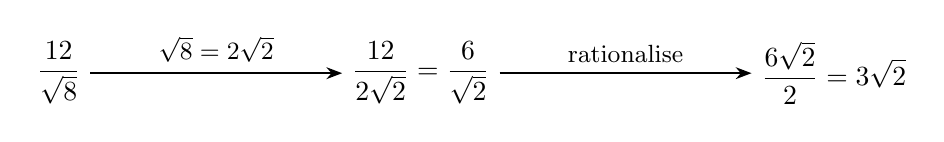
\begin{tikzpicture}[>={Stealth[length=2mm]},node distance=1.5cm and 3.2cm]
\node (s0) {$\displaystyle \frac{12}{\sqrt8}$};
\node (s1) [right=of s0] {$\displaystyle \frac{12}{2\sqrt2}=\frac{6}{\sqrt2}$};
\node (s2) [right=of s1] {$\displaystyle \frac{6\sqrt2}{2}=3\sqrt2$};
\draw[->,thick] (s0) -- (s1) node[midway,above,font=\small]{$\sqrt8=2\sqrt2$};
\draw[->,thick] (s1) -- (s2) node[midway,above,font=\small]{rationalise};
\end{tikzpicture}
}
\end{center}
\small Solution flow: each arrow applies one step.\normalsize

\medskip\hrule

\section*{Rationalising the Denominator 44\quad\small\texttt{(a6-044)}}
\addcontentsline{toc}{section}{Rationalising the Denominator 44 (a6-044)}
\textit{Difficulty: Foundation \quad\textbar\quad Marks: 4}

\question{Solve the equation \( 10 = (\sqrt{3} - 1)x \), giving your answer in the form \( a + b\sqrt{3} \) where \( a \) and \( b \) are integers.}

\textbf{Worked solution.}

\textit{Step 1: Divide both sides by \( \sqrt{3} - 1 \).}
\[\begin{gathered}
x = \frac{10}{\sqrt{3} - 1}
\end{gathered}\]
Isolate \( x \).

\textit{Step 2: Multiply top and bottom by the conjugate \( \sqrt{3} + 1 \).}
\[\begin{gathered}
x = \frac{10(\sqrt{3} + 1)}{(\sqrt{3} - 1)(\sqrt{3} + 1)} = \frac{10(\sqrt{3} + 1)}{3 - 1}
\end{gathered}\]
\( (\sqrt{3})^2 - 1 = 2 \).

\textit{Step 3: Simplify.}
\[\begin{gathered}
x = \frac{10(\sqrt{3} + 1)}{2} = 5(\sqrt{3} + 1) = 5 + 5\sqrt{3}
\end{gathered}\]
\( \frac{10}{2} = 5 \), then expand the bracket.

\begin{answerbox}
\textbf{Final answer:}\quad \(\displaystyle x = 5 + 5\sqrt{3}\)
\end{answerbox}
\textbf{Diagram.}

\begin{center}
\resizebox{\ifdim\width>\linewidth \linewidth\else \width\fi}{!}{%
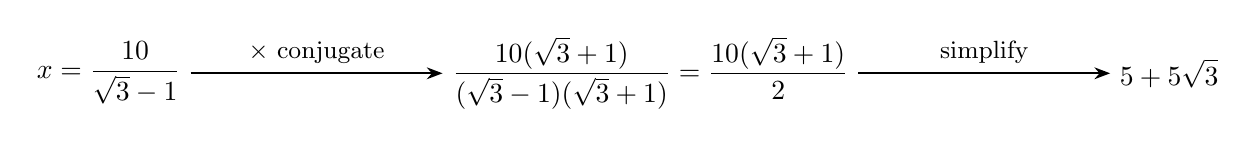
\begin{tikzpicture}[>={Stealth[length=2mm]},node distance=1.5cm and 3.2cm]
\node (s0) {$\displaystyle x=\frac{10}{\sqrt3-1}$};
\node (s1) [right=of s0] {$\displaystyle \frac{10(\sqrt3+1)}{(\sqrt3-1)(\sqrt3+1)}=\frac{10(\sqrt3+1)}{2}$};
\node (s2) [right=of s1] {$\displaystyle 5+5\sqrt3$};
\draw[->,thick] (s0) -- (s1) node[midway,above,font=\small]{$\times$ conjugate};
\draw[->,thick] (s1) -- (s2) node[midway,above,font=\small]{simplify};
\end{tikzpicture}
}
\end{center}
\small Solution flow: each arrow applies one step.\normalsize

\medskip\hrule

\section*{Rationalising the Denominator 45\quad\small\texttt{(a6-045)}}
\addcontentsline{toc}{section}{Rationalising the Denominator 45 (a6-045)}
\textit{Difficulty: Foundation \quad\textbar\quad Marks: 5}

\question{Solve the equation \( 4 + \sqrt{5} = (2 - \sqrt{5})y \), giving your answer in the form \( p + q\sqrt{5} \) where \( p \) and \( q \) are integers.}

\textbf{Worked solution.}

\textit{Step 1: Divide both sides by \( 2 - \sqrt{5} \).}
\[\begin{gathered}
y = \frac{4 + \sqrt{5}}{2 - \sqrt{5}}
\end{gathered}\]
Isolate \( y \).

\textit{Step 2: Multiply top and bottom by the conjugate \( 2 + \sqrt{5} \).}
\[\begin{gathered}
y = \frac{(4 + \sqrt{5})(2 + \sqrt{5})}{(2 - \sqrt{5})(2 + \sqrt{5})}
\end{gathered}\]
Use the conjugate to eliminate the surd from the denominator.

\textit{Step 3: Expand the numerator and denominator.}
\[\begin{gathered}
y = \frac{8 + 4\sqrt{5} + 2\sqrt{5} + 5}{4 - 5} = \frac{13 + 6\sqrt{5}}{-1}
\end{gathered}\]
Numerator: \( 8 + 6\sqrt{5} + 5 = 13 + 6\sqrt{5} \). Denominator: \( 4 - 5 = -1 \).

\textit{Step 4: Simplify.}
\[\begin{gathered}
y = -13 - 6\sqrt{5}
\end{gathered}\]
Dividing by \( -1 \) negates each term.

\begin{answerbox}
\textbf{Final answer:}\quad \(\displaystyle y = -13 - 6\sqrt{5}\)
\end{answerbox}
\textbf{Diagram.}

\begin{center}
\resizebox{\ifdim\width>\linewidth \linewidth\else \width\fi}{!}{%
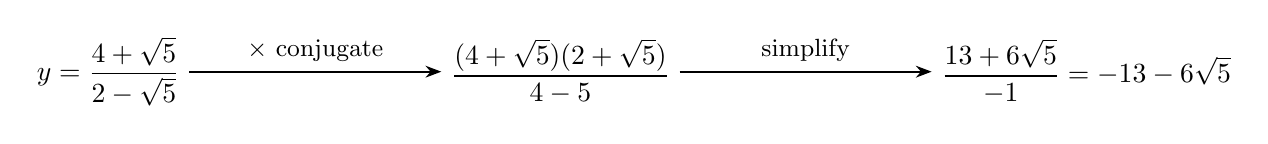
\begin{tikzpicture}[>={Stealth[length=2mm]},node distance=1.5cm and 3.2cm]
\node (s0) {$\displaystyle y=\frac{4+\sqrt5}{2-\sqrt5}$};
\node (s1) [right=of s0] {$\displaystyle \frac{(4+\sqrt5)(2+\sqrt5)}{4-5}$};
\node (s2) [right=of s1] {$\displaystyle \frac{13+6\sqrt5}{-1}=-13-6\sqrt5$};
\draw[->,thick] (s0) -- (s1) node[midway,above,font=\small]{$\times$ conjugate};
\draw[->,thick] (s1) -- (s2) node[midway,above,font=\small]{simplify};
\end{tikzpicture}
}
\end{center}
\small Solution flow: each arrow applies one step.\normalsize

\medskip\hrule

\section*{Rationalising the Denominator 46\quad\small\texttt{(a6-046)}}
\addcontentsline{toc}{section}{Rationalising the Denominator 46 (a6-046)}
\textit{Difficulty: Foundation \quad\textbar\quad Marks: 5}

\question{A rectangle has an area of \( (3 + \sqrt{5}) \) cm\(^2\) and a width of \( (\sqrt{5} - 1) \) cm. Find the length of the rectangle. Give your answer in the form \( a + b\sqrt{5} \), where \( a \) and \( b \) are integers.}

\textbf{Worked solution.}

\textit{Step 1: Use the formula \( \text{length} = \frac{\text{area}}{\text{width}} \).}
\[\begin{gathered}
\text{length} = \frac{3 + \sqrt{5}}{\sqrt{5} - 1}
\end{gathered}\]
Divide the area by the width.

\textit{Step 2: Multiply top and bottom by the conjugate \( \sqrt{5} + 1 \).}
\[\begin{gathered}
\frac{(3 + \sqrt{5})(\sqrt{5} + 1)}{(\sqrt{5} - 1)(\sqrt{5} + 1)}
\end{gathered}\]
The conjugate eliminates the surd from the denominator.

\textit{Step 3: Expand the numerator and denominator.}
\[\begin{gathered}
\frac{3\sqrt{5} + 3 + 5 + \sqrt{5}}{5 - 1} = \frac{8 + 4\sqrt{5}}{4}
\end{gathered}\]
Numerator: \( 3\sqrt{5} + 3 + \sqrt{5} \times \sqrt{5} + \sqrt{5} = 3\sqrt{5} + 3 + 5 + \sqrt{5} = 8 + 4\sqrt{5} \). Denominator: \( 5 - 1 = 4 \).

\textit{Step 4: Simplify.}
\[\begin{gathered}
2 + \sqrt{5}
\end{gathered}\]
Divide each term by 4.

\begin{answerbox}
\textbf{Final answer:}\quad \(\displaystyle (2 + \sqrt{5})\) cm
\end{answerbox}
\textbf{Diagram.}

\begin{center}
\resizebox{\ifdim\width>\linewidth \linewidth\else \width\fi}{!}{%
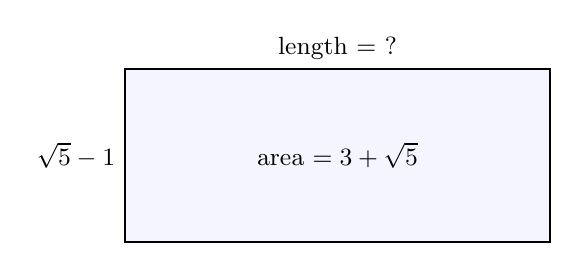
\begin{tikzpicture}[font=\small]
\draw[thick,fill=blue!4] (0,0) rectangle (5.4,2.2);
\node[above] at (2.7,2.2) {length $=\ ?$};
\node[left] at (0,1.1) {$\sqrt5-1$};
\node at (2.7,1.1) {area $=3+\sqrt5$};
\end{tikzpicture}
}
\end{center}
\small length $=$ area $\div$ width $=\dfrac{3+\sqrt5}{\sqrt5-1}$; multiplying by the conjugate $\dfrac{\sqrt5+1}{\sqrt5+1}$ gives $\dfrac{(3+\sqrt5)(\sqrt5+1)}{4}=\dfrac{8+4\sqrt5}{4}=2+\sqrt5$ cm.\normalsize

\medskip\hrule

\section*{Rationalising the Denominator 47\quad\small\texttt{(a6-047)}}
\addcontentsline{toc}{section}{Rationalising the Denominator 47 (a6-047)}
\textit{Difficulty: Foundation \quad\textbar\quad Marks: 3}

\question{Rationalise the denominator: \( \frac{1}{\sqrt{2} + \sqrt{3}} \)}

\textbf{Worked solution.}

\textit{Step 1: Multiply top and bottom by the conjugate \( \sqrt{2} - \sqrt{3} \).}
\[\begin{gathered}
\frac{\sqrt{2} - \sqrt{3}}{(\sqrt{2} + \sqrt{3})(\sqrt{2} - \sqrt{3})}
\end{gathered}\]
Use the conjugate to eliminate surds from the denominator.

\textit{Step 2: Expand the denominator.}
\[\begin{gathered}
\frac{\sqrt{2} - \sqrt{3}}{2 - 3} = \frac{\sqrt{2} - \sqrt{3}}{-1}
\end{gathered}\]
\( (\sqrt{2})^2 - (\sqrt{3})^2 = 2 - 3 = -1 \).

\textit{Step 3: Simplify by multiplying through by \( -1 \).}
\[\begin{gathered}
\sqrt{3} - \sqrt{2}
\end{gathered}\]
Dividing by \( -1 \) flips the signs.

\begin{answerbox}
\textbf{Final answer:}\quad \(\displaystyle \sqrt{3} - \sqrt{2}\)
\end{answerbox}
\textbf{Diagram.}

\begin{center}
\resizebox{\ifdim\width>\linewidth \linewidth\else \width\fi}{!}{%
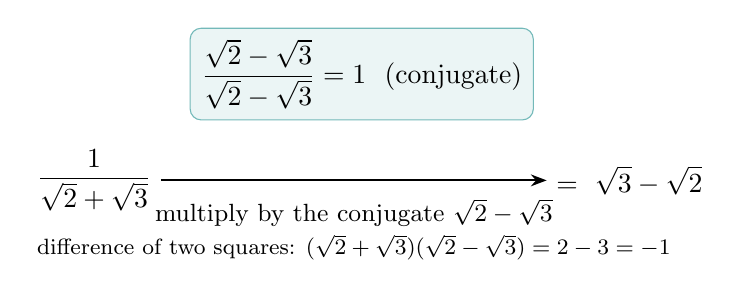
\begin{tikzpicture}[>={Stealth[length=2mm]}]
\node[draw=teal!55,rounded corners,fill=teal!8,inner sep=4pt] (rule) at (3.4,1.35) {$\displaystyle \frac{\sqrt2-\sqrt3}{\sqrt2-\sqrt3}=1$ \ (conjugate)};
\node (L) at (0,0) {$\displaystyle \frac{1}{\sqrt2+\sqrt3}$};
\node (R) at (6.8,0) {$\displaystyle =\ \sqrt3-\sqrt2$};
\draw[->,thick] (L) -- (R) node[midway,below=3pt,font=\small,align=center]{multiply by the conjugate $\sqrt2-\sqrt3$\\[1pt]\footnotesize difference of two squares: $(\sqrt2+\sqrt3)(\sqrt2-\sqrt3)=2-3=-1$};
\end{tikzpicture}
}
\end{center}
\small Multiply by the conjugate over itself. The denominator is then a difference of two squares, $(A+B)(A-B)=A^{2}-B^{2}$, so every surd cancels and the denominator becomes rational.\normalsize

\medskip\hrule

\section*{Rationalising the Denominator 48\quad\small\texttt{(a6-048)}}
\addcontentsline{toc}{section}{Rationalising the Denominator 48 (a6-048)}
\textit{Difficulty: Foundation \quad\textbar\quad Marks: 4}

\question{Express in the form \( p + q\sqrt{r} \) where \( r \) is an integer, and \( p \) and \( q \) are integers or fractions: \( \frac{\sqrt{6} + \sqrt{2}}{\sqrt{6} - \sqrt{2}} \)}

\textbf{Worked solution.}

\textit{Step 1: Multiply top and bottom by the conjugate \( \sqrt{6} + \sqrt{2} \).}
\[\begin{gathered}
\frac{(\sqrt{6} + \sqrt{2})(\sqrt{6} + \sqrt{2})}{(\sqrt{6} - \sqrt{2})(\sqrt{6} + \sqrt{2})}
\end{gathered}\]
Use the conjugate of the denominator.

\textit{Step 2: Expand the numerator and denominator.}
\[\begin{gathered}
\frac{6 + 2\sqrt{12} + 2}{6 - 2} = \frac{8 + 2\sqrt{12}}{4}
\end{gathered}\]
Numerator: \( (\sqrt{6})^2 + 2\sqrt{6}\sqrt{2} + (\sqrt{2})^2 = 6 + 2\sqrt{12} + 2 = 8 + 2\sqrt{12} \). Denominator: \( 6 - 2 = 4 \).

\textit{Step 3: Simplify \( \sqrt{12} = 2\sqrt{3} \).}
\[\begin{gathered}
\frac{8 + 4\sqrt{3}}{4} = 2 + \sqrt{3}
\end{gathered}\]
Divide each term by 4.

\begin{answerbox}
\textbf{Final answer:}\quad \(\displaystyle 2 + \sqrt{3}\)
\end{answerbox}
\textbf{Diagram.}

\begin{center}
\resizebox{\ifdim\width>\linewidth \linewidth\else \width\fi}{!}{%
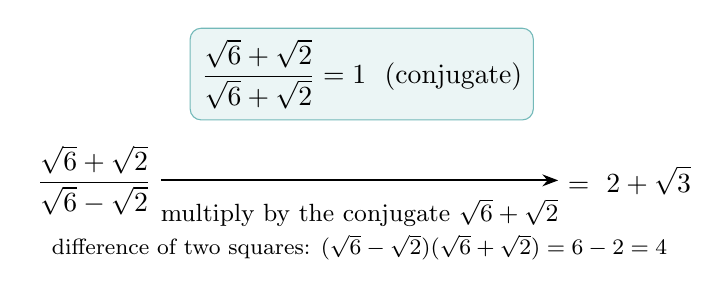
\begin{tikzpicture}[>={Stealth[length=2mm]}]
\node[draw=teal!55,rounded corners,fill=teal!8,inner sep=4pt] (rule) at (3.4,1.35) {$\displaystyle \frac{\sqrt6+\sqrt2}{\sqrt6+\sqrt2}=1$ \ (conjugate)};
\node (L) at (0,0) {$\displaystyle \frac{\sqrt6+\sqrt2}{\sqrt6-\sqrt2}$};
\node (R) at (6.8,0) {$\displaystyle =\ 2+\sqrt3$};
\draw[->,thick] (L) -- (R) node[midway,below=3pt,font=\small,align=center]{multiply by the conjugate $\sqrt6+\sqrt2$\\[1pt]\footnotesize difference of two squares: $(\sqrt6-\sqrt2)(\sqrt6+\sqrt2)=6-2=4$};
\end{tikzpicture}
}
\end{center}
\small Multiply by the conjugate over itself. The denominator is then a difference of two squares, $(A+B)(A-B)=A^{2}-B^{2}$, so every surd cancels and the denominator becomes rational.\normalsize

\medskip\hrule

\section*{Rationalising the Denominator 49\quad\small\texttt{(a6-049)}}
\addcontentsline{toc}{section}{Rationalising the Denominator 49 (a6-049)}
\textit{Difficulty: Foundation \quad\textbar\quad Marks: 4}

\question{Rationalise the denominator: \( \frac{\sqrt{2}}{3\sqrt{2} + 1} \)}

\textbf{Worked solution.}

\textit{Step 1: Multiply top and bottom by the conjugate \( 3\sqrt{2} - 1 \).}
\[\begin{gathered}
\frac{\sqrt{2}(3\sqrt{2} - 1)}{(3\sqrt{2} + 1)(3\sqrt{2} - 1)}
\end{gathered}\]
Flip the sign between the terms.

\textit{Step 2: Expand the numerator and denominator.}
\[\begin{gathered}
\frac{3 \times 2 - \sqrt{2}}{9 \times 2 - 1} = \frac{6 - \sqrt{2}}{17}
\end{gathered}\]
Numerator: \( \sqrt{2} \times 3\sqrt{2} = 6 \) and \( \sqrt{2} \times (-1) = -\sqrt{2} \). Denominator: \( (3\sqrt{2})^2 - 1 = 18 - 1 = 17 \).

\begin{answerbox}
\textbf{Final answer:}\quad \(\displaystyle \frac{6 - \sqrt{2}}{17}\)
\end{answerbox}
\textbf{Diagram.}

\begin{center}
\resizebox{\ifdim\width>\linewidth \linewidth\else \width\fi}{!}{%
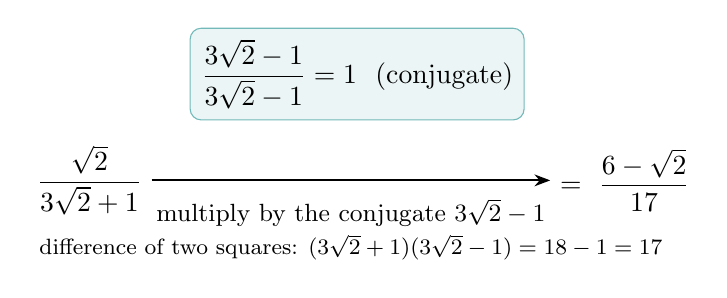
\begin{tikzpicture}[>={Stealth[length=2mm]}]
\node[draw=teal!55,rounded corners,fill=teal!8,inner sep=4pt] (rule) at (3.4,1.35) {$\displaystyle \frac{3\sqrt2-1}{3\sqrt2-1}=1$ \ (conjugate)};
\node (L) at (0,0) {$\displaystyle \frac{\sqrt2}{3\sqrt2+1}$};
\node (R) at (6.8,0) {$\displaystyle =\ \frac{6-\sqrt2}{17}$};
\draw[->,thick] (L) -- (R) node[midway,below=3pt,font=\small,align=center]{multiply by the conjugate $3\sqrt2-1$\\[1pt]\footnotesize difference of two squares: $(3\sqrt2+1)(3\sqrt2-1)=18-1=17$};
\end{tikzpicture}
}
\end{center}
\small Multiply by the conjugate over itself. The denominator is then a difference of two squares, $(A+B)(A-B)=A^{2}-B^{2}$, so every surd cancels and the denominator becomes rational.\normalsize

\medskip\hrule

\section*{Rationalising the Denominator 50\quad\small\texttt{(a6-050)}}
\addcontentsline{toc}{section}{Rationalising the Denominator 50 (a6-050)}
\textit{Difficulty: Foundation \quad\textbar\quad Marks: 2}

\question{Show that \( \frac{12}{\sqrt{3}} = 4\sqrt{3} \).}

\textbf{Worked solution.}

\textit{Step 1: Multiply the top and bottom by \( \sqrt{3} \).}
\[\begin{gathered}
\frac{12}{\sqrt{3}} \times \frac{\sqrt{3}}{\sqrt{3}} = \frac{12\sqrt{3}}{3}
\end{gathered}\]
\( \sqrt{3} \times \sqrt{3} = 3 \).

\textit{Step 2: Simplify.}
\[\begin{gathered}
\frac{12\sqrt{3}}{3} = 4\sqrt{3}
\end{gathered}\]
\( 12 \div 3 = 4 \), showing the result.

\begin{answerbox}
\textbf{Final answer:}\quad \(\displaystyle 4\sqrt{3} ( shown )\)
\end{answerbox}
\textbf{Diagram.}

\begin{center}
\resizebox{\ifdim\width>\linewidth \linewidth\else \width\fi}{!}{%
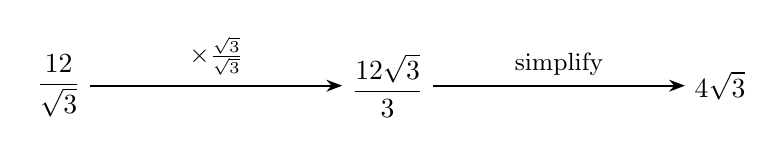
\begin{tikzpicture}[>={Stealth[length=2mm]},node distance=1.5cm and 3.2cm]
\node (s0) {$\displaystyle \frac{12}{\sqrt3}$};
\node (s1) [right=of s0] {$\displaystyle \frac{12\sqrt3}{3}$};
\node (s2) [right=of s1] {$\displaystyle 4\sqrt3$};
\draw[->,thick] (s0) -- (s1) node[midway,above,font=\small]{$\times\tfrac{\sqrt3}{\sqrt3}$};
\draw[->,thick] (s1) -- (s2) node[midway,above,font=\small]{simplify};
\end{tikzpicture}
}
\end{center}
\small Solution flow: each arrow applies one step.\normalsize

\medskip\hrule

\section*{Rationalising the Denominator 51\quad\small\texttt{(a6-051)}}
\addcontentsline{toc}{section}{Rationalising the Denominator 51 (a6-051)}
\textit{Difficulty: Foundation \quad\textbar\quad Marks: 2}

\question{Rationalise and simplify: \( \frac{\sqrt{27}}{\sqrt{3}} \)}

\textbf{Worked solution.}

\textit{Step 1: Combine under a single root.}
\[\begin{gathered}
\sqrt{\frac{27}{3}} = \sqrt{9}
\end{gathered}\]
Use \( \frac{\sqrt{a}}{\sqrt{b}} = \sqrt{\frac{a}{b}} \).

\textit{Step 2: Evaluate.}
\[\begin{gathered}
3
\end{gathered}\]
\( \sqrt{9} = 3 \).

\begin{answerbox}
\textbf{Final answer:}\quad \(\displaystyle 3\)
\end{answerbox}
\textbf{Diagram.}

\begin{center}
\resizebox{\ifdim\width>\linewidth \linewidth\else \width\fi}{!}{%
\begin{tikzpicture}[>={Stealth[length=2mm]},node distance=1.5cm and 3.2cm]
\node (s0) {$\displaystyle \frac{\sqrt{27}}{\sqrt3}$};
\node (s1) [right=of s0] {$\displaystyle \sqrt{\tfrac{27}{3}}=\sqrt9$};
\node (s2) [right=of s1] {$\displaystyle 3$};
\draw[->,thick] (s0) -- (s1) node[midway,above,font=\small]{one root};
\draw[->,thick] (s1) -- (s2) node[midway,above,font=\small]{evaluate};
\end{tikzpicture}
}
\end{center}
\small Solution flow: each arrow applies one step.\normalsize

\medskip\hrule

\section*{Rationalising the Denominator 52\quad\small\texttt{(a6-052)}}
\addcontentsline{toc}{section}{Rationalising the Denominator 52 (a6-052)}
\textit{Difficulty: Foundation \quad\textbar\quad Marks: 4}

\question{Express in the form \( a + b\sqrt{k} \) where \( a \), \( b \) and \( k \) are integers: \( \frac{11}{2\sqrt{3} - 1} \)}

\textbf{Worked solution.}

\textit{Step 1: Multiply top and bottom by the conjugate \( 2\sqrt{3} + 1 \).}
\[\begin{gathered}
\frac{11(2\sqrt{3} + 1)}{(2\sqrt{3} - 1)(2\sqrt{3} + 1)}
\end{gathered}\]
Use the conjugate to eliminate the surd.

\textit{Step 2: Expand the denominator.}
\[\begin{gathered}
\frac{11(2\sqrt{3} + 1)}{12 - 1} = \frac{11(2\sqrt{3} + 1)}{11}
\end{gathered}\]
\( (2\sqrt{3})^2 - 1 = 12 - 1 = 11 \).

\textit{Step 3: Cancel the common factor of 11.}
\[\begin{gathered}
2\sqrt{3} + 1 = 1 + 2\sqrt{3}
\end{gathered}\]
Giving \( a = 1 \), \( b = 2 \), \( k = 3 \).

\begin{answerbox}
\textbf{Final answer:}\quad \(\displaystyle 1 + 2\sqrt{3}\)
\end{answerbox}
\textbf{Diagram.}

\begin{center}
\resizebox{\ifdim\width>\linewidth \linewidth\else \width\fi}{!}{%
\begin{tikzpicture}[>={Stealth[length=2mm]}]
\node[draw=teal!55,rounded corners,fill=teal!8,inner sep=4pt] (rule) at (3.4,1.35) {$\displaystyle \frac{2\sqrt3+1}{2\sqrt3+1}=1$ \ (conjugate)};
\node (L) at (0,0) {$\displaystyle \frac{11}{2\sqrt3-1}$};
\node (R) at (6.8,0) {$\displaystyle =\ 1+2\sqrt3$};
\draw[->,thick] (L) -- (R) node[midway,below=3pt,font=\small,align=center]{multiply by the conjugate $2\sqrt3+1$\\[1pt]\footnotesize difference of two squares: $(2\sqrt3-1)(2\sqrt3+1)=12-1=11$};
\end{tikzpicture}
}
\end{center}
\small Multiply by the conjugate over itself. The denominator is then a difference of two squares, $(A+B)(A-B)=A^{2}-B^{2}$, so every surd cancels and the denominator becomes rational.\normalsize

\medskip\hrule

\section*{Rationalising the Denominator 53\quad\small\texttt{(a6-053)}}
\addcontentsline{toc}{section}{Rationalising the Denominator 53 (a6-053)}
\textit{Difficulty: Foundation \quad\textbar\quad Marks: 4}

\question{Express in the form \( a + b\sqrt{k} \) where \( a \), \( b \) and \( k \) are integers: \( \frac{11}{2\sqrt{5} + 3} \)}

\textbf{Worked solution.}

\textit{Step 1: Multiply top and bottom by the conjugate \( 2\sqrt{5} - 3 \).}
\[\begin{gathered}
\frac{11(2\sqrt{5} - 3)}{(2\sqrt{5} + 3)(2\sqrt{5} - 3)}
\end{gathered}\]
Flip the sign between the terms.

\textit{Step 2: Expand the denominator.}
\[\begin{gathered}
\frac{11(2\sqrt{5} - 3)}{20 - 9} = \frac{11(2\sqrt{5} - 3)}{11}
\end{gathered}\]
\( (2\sqrt{5})^2 - 3^2 = 20 - 9 = 11 \).

\textit{Step 3: Cancel the common factor of 11.}
\[\begin{gathered}
2\sqrt{5} - 3 = -3 + 2\sqrt{5}
\end{gathered}\]
Giving \( a = -3 \), \( b = 2 \), \( k = 5 \).

\begin{answerbox}
\textbf{Final answer:}\quad \(\displaystyle -3 + 2\sqrt{5}\)
\end{answerbox}
\textbf{Diagram.}

\begin{center}
\resizebox{\ifdim\width>\linewidth \linewidth\else \width\fi}{!}{%
\begin{tikzpicture}[>={Stealth[length=2mm]}]
\node[draw=teal!55,rounded corners,fill=teal!8,inner sep=4pt] (rule) at (3.4,1.35) {$\displaystyle \frac{2\sqrt5-3}{2\sqrt5-3}=1$ \ (conjugate)};
\node (L) at (0,0) {$\displaystyle \frac{11}{2\sqrt5+3}$};
\node (R) at (6.8,0) {$\displaystyle =\ -3+2\sqrt5$};
\draw[->,thick] (L) -- (R) node[midway,below=3pt,font=\small,align=center]{multiply by the conjugate $2\sqrt5-3$\\[1pt]\footnotesize difference of two squares: $(2\sqrt5+3)(2\sqrt5-3)=20-9=11$};
\end{tikzpicture}
}
\end{center}
\small Multiply by the conjugate over itself. The denominator is then a difference of two squares, $(A+B)(A-B)=A^{2}-B^{2}$, so every surd cancels and the denominator becomes rational.\normalsize

\medskip\hrule

\section*{Rationalising the Denominator 54\quad\small\texttt{(a6-054)}}
\addcontentsline{toc}{section}{Rationalising the Denominator 54 (a6-054)}
\textit{Difficulty: Foundation \quad\textbar\quad Marks: 2}

\question{Simplify, giving your answer in the form \( p\sqrt{q} \) where \( p \) and \( q \) are integers: \( \frac{25}{\sqrt{5}} \)}

\textbf{Worked solution.}

\textit{Step 1: Multiply the top and bottom by \( \sqrt{5} \).}
\[\begin{gathered}
\frac{25\sqrt{5}}{5}
\end{gathered}\]
\( \sqrt{5} \times \sqrt{5} = 5 \).

\textit{Step 2: Simplify.}
\[\begin{gathered}
5\sqrt{5}
\end{gathered}\]
\( 25 \div 5 = 5 \).

\begin{answerbox}
\textbf{Final answer:}\quad \(\displaystyle 5\sqrt{5}\)
\end{answerbox}
\textbf{Diagram.}

\begin{center}
\resizebox{\ifdim\width>\linewidth \linewidth\else \width\fi}{!}{%
\begin{tikzpicture}[>={Stealth[length=2mm]}]
\node[draw=teal!55,rounded corners,fill=teal!8,inner sep=4pt] (rule) at (3.4,1.3) {$\displaystyle \frac{\sqrt5}{\sqrt5}=1$};
\node (L) at (0,0) {$\displaystyle \frac{25}{\sqrt5}$};
\node (R) at (6.8,0) {$\displaystyle =\ 5\sqrt5$};
\draw[->,thick] (L) -- (R) node[midway,below=3pt,font=\small,align=center]{multiply top and bottom by $\sqrt5$\\[1pt]\footnotesize denominator: $\sqrt5\times\sqrt5=5$};
\end{tikzpicture}
}
\end{center}
\small Then $\frac{25\sqrt5}{5}=5\sqrt5$. Multiply by $\frac{\sqrt{a}}{\sqrt{a}}=1$: this leaves the value unchanged but clears the surd from the denominator.\normalsize

\medskip\hrule

\section*{Rationalising the Denominator 55\quad\small\texttt{(a6-055)}}
\addcontentsline{toc}{section}{Rationalising the Denominator 55 (a6-055)}
\textit{Difficulty: Foundation \quad\textbar\quad Marks: 2}

\question{Simplify, giving your answer in the form \( p\sqrt{q} \) where \( p \) and \( q \) are integers: \( \frac{18}{\sqrt{6}} \)}

\textbf{Worked solution.}

\textit{Step 1: Multiply the top and bottom by \( \sqrt{6} \).}
\[\begin{gathered}
\frac{18\sqrt{6}}{6}
\end{gathered}\]
\( \sqrt{6} \times \sqrt{6} = 6 \).

\textit{Step 2: Simplify.}
\[\begin{gathered}
3\sqrt{6}
\end{gathered}\]
\( 18 \div 6 = 3 \).

\begin{answerbox}
\textbf{Final answer:}\quad \(\displaystyle 3\sqrt{6}\)
\end{answerbox}
\textbf{Diagram.}

\begin{center}
\resizebox{\ifdim\width>\linewidth \linewidth\else \width\fi}{!}{%
\begin{tikzpicture}[>={Stealth[length=2mm]}]
\node[draw=teal!55,rounded corners,fill=teal!8,inner sep=4pt] (rule) at (3.4,1.3) {$\displaystyle \frac{\sqrt6}{\sqrt6}=1$};
\node (L) at (0,0) {$\displaystyle \frac{18}{\sqrt6}$};
\node (R) at (6.8,0) {$\displaystyle =\ 3\sqrt6$};
\draw[->,thick] (L) -- (R) node[midway,below=3pt,font=\small,align=center]{multiply top and bottom by $\sqrt6$\\[1pt]\footnotesize denominator: $\sqrt6\times\sqrt6=6$};
\end{tikzpicture}
}
\end{center}
\small Then $\frac{18\sqrt6}{6}=3\sqrt6$. Multiply by $\frac{\sqrt{a}}{\sqrt{a}}=1$: this leaves the value unchanged but clears the surd from the denominator.\normalsize

\medskip\hrule

\section*{Rationalising the Denominator 56\quad\small\texttt{(a6-056)}}
\addcontentsline{toc}{section}{Rationalising the Denominator 56 (a6-056)}
\textit{Difficulty: Foundation \quad\textbar\quad Marks: 2}

\question{Rationalise and simplify: \( \frac{\sqrt{48}}{\sqrt{6}} \)}

\textbf{Worked solution.}

\textit{Step 1: Combine the surds under a single root.}
\[\begin{gathered}
\sqrt{\frac{48}{6}} = \sqrt{8}
\end{gathered}\]
Use the quotient rule for surds.

\textit{Step 2: Simplify \( \sqrt{8} \).}
\[\begin{gathered}
\sqrt{4 \times 2} = 2\sqrt{2}
\end{gathered}\]
4 is the largest square factor of 8.

\begin{answerbox}
\textbf{Final answer:}\quad \(\displaystyle 2\sqrt{2}\)
\end{answerbox}
\textbf{Diagram.}

\begin{center}
\resizebox{\ifdim\width>\linewidth \linewidth\else \width\fi}{!}{%
\begin{tikzpicture}[>={Stealth[length=2mm]},node distance=1.5cm and 3.2cm]
\node (s0) {$\displaystyle \frac{\sqrt{48}}{\sqrt6}$};
\node (s1) [right=of s0] {$\displaystyle \sqrt{\tfrac{48}{6}}=\sqrt8$};
\node (s2) [right=of s1] {$\displaystyle 2\sqrt2$};
\draw[->,thick] (s0) -- (s1) node[midway,above,font=\small]{one root};
\draw[->,thick] (s1) -- (s2) node[midway,above,font=\small]{simplify};
\end{tikzpicture}
}
\end{center}
\small Solution flow: each arrow applies one step.\normalsize

\medskip\hrule

\section*{Rationalising the Denominator 57\quad\small\texttt{(a6-057)}}
\addcontentsline{toc}{section}{Rationalising the Denominator 57 (a6-057)}
\textit{Difficulty: Foundation \quad\textbar\quad Marks: 3}

\question{Express in the form \( a + b\sqrt{k} \) where \( a \), \( b \) and \( k \) are integers: \( \frac{2}{3 - \sqrt{7}} \)}

\textbf{Worked solution.}

\textit{Step 1: Multiply top and bottom by the conjugate \( 3 + \sqrt{7} \).}
\[\begin{gathered}
\frac{2(3 + \sqrt{7})}{(3 - \sqrt{7})(3 + \sqrt{7})}
\end{gathered}\]
Flip the sign between the terms.

\textit{Step 2: Expand the denominator.}
\[\begin{gathered}
\frac{2(3 + \sqrt{7})}{9 - 7} = \frac{2(3 + \sqrt{7})}{2}
\end{gathered}\]
\( 9 - 7 = 2 \).

\textit{Step 3: Cancel.}
\[\begin{gathered}
3 + \sqrt{7}
\end{gathered}\]
The 2s cancel exactly.

\begin{answerbox}
\textbf{Final answer:}\quad \(\displaystyle 3 + \sqrt{7}\)
\end{answerbox}
\textbf{Diagram.}

\begin{center}
\resizebox{\ifdim\width>\linewidth \linewidth\else \width\fi}{!}{%
\begin{tikzpicture}[>={Stealth[length=2mm]}]
\node[draw=teal!55,rounded corners,fill=teal!8,inner sep=4pt] (rule) at (3.4,1.35) {$\displaystyle \frac{3+\sqrt7}{3+\sqrt7}=1$ \ (conjugate)};
\node (L) at (0,0) {$\displaystyle \frac{2}{3-\sqrt7}$};
\node (R) at (6.8,0) {$\displaystyle =\ 3+\sqrt7$};
\draw[->,thick] (L) -- (R) node[midway,below=3pt,font=\small,align=center]{multiply by the conjugate $3+\sqrt7$\\[1pt]\footnotesize difference of two squares: $(3-\sqrt7)(3+\sqrt7)=9-7=2$};
\end{tikzpicture}
}
\end{center}
\small Multiply by the conjugate over itself. The denominator is then a difference of two squares, $(A+B)(A-B)=A^{2}-B^{2}$, so every surd cancels and the denominator becomes rational.\normalsize

\medskip\hrule

\section*{Rationalising the Denominator 58\quad\small\texttt{(a6-058)}}
\addcontentsline{toc}{section}{Rationalising the Denominator 58 (a6-058)}
\textit{Difficulty: Foundation \quad\textbar\quad Marks: 4}

\question{Express in the form \( k(\sqrt{x} \pm \sqrt{y}) \), where \( x \) and \( y \) are integers and \( k \) is an integer or fraction: \( \frac{15}{\sqrt{6} + \sqrt{3}} \)}

\textbf{Worked solution.}

\textit{Step 1: Multiply top and bottom by the conjugate \( \sqrt{6} - \sqrt{3} \).}
\[\begin{gathered}
\frac{15(\sqrt{6} - \sqrt{3})}{(\sqrt{6} + \sqrt{3})(\sqrt{6} - \sqrt{3})}
\end{gathered}\]
Switch the sign between the surds.

\textit{Step 2: Expand the denominator.}
\[\begin{gathered}
\frac{15(\sqrt{6} - \sqrt{3})}{6 - 3} = \frac{15(\sqrt{6} - \sqrt{3})}{3}
\end{gathered}\]
\( 6 - 3 = 3 \).

\textit{Step 3: Simplify.}
\[\begin{gathered}
5(\sqrt{6} - \sqrt{3})
\end{gathered}\]
\( \frac{15}{3} = 5 \).

\begin{answerbox}
\textbf{Final answer:}\quad \(\displaystyle 5(\sqrt{6} - \sqrt{3})\)
\end{answerbox}
\textbf{Diagram.}

\begin{center}
\resizebox{\ifdim\width>\linewidth \linewidth\else \width\fi}{!}{%
\begin{tikzpicture}[>={Stealth[length=2mm]}]
\node[draw=teal!55,rounded corners,fill=teal!8,inner sep=4pt] (rule) at (3.4,1.35) {$\displaystyle \frac{\sqrt6-\sqrt3}{\sqrt6-\sqrt3}=1$ \ (conjugate)};
\node (L) at (0,0) {$\displaystyle \frac{15}{\sqrt6+\sqrt3}$};
\node (R) at (6.8,0) {$\displaystyle =\ 5(\sqrt6-\sqrt3)$};
\draw[->,thick] (L) -- (R) node[midway,below=3pt,font=\small,align=center]{multiply by the conjugate $\sqrt6-\sqrt3$\\[1pt]\footnotesize difference of two squares: $(\sqrt6+\sqrt3)(\sqrt6-\sqrt3)=6-3=3$};
\end{tikzpicture}
}
\end{center}
\small Multiply by the conjugate over itself. The denominator is then a difference of two squares, $(A+B)(A-B)=A^{2}-B^{2}$, so every surd cancels and the denominator becomes rational.\normalsize

\medskip\hrule

\section*{Rationalising the Denominator 59\quad\small\texttt{(a6-059)}}
\addcontentsline{toc}{section}{Rationalising the Denominator 59 (a6-059)}
\textit{Difficulty: Foundation \quad\textbar\quad Marks: 4}

\question{Rationalise the denominator: \( \frac{\sqrt{3}}{\sqrt{15} - \sqrt{6}} \)}

\textbf{Worked solution.}

\textit{Step 1: Multiply top and bottom by the conjugate \( \sqrt{15} + \sqrt{6} \).}
\[\begin{gathered}
\frac{\sqrt{3}(\sqrt{15} + \sqrt{6})}{(\sqrt{15} - \sqrt{6})(\sqrt{15} + \sqrt{6})}
\end{gathered}\]
Use the conjugate to eliminate surds from the denominator.

\textit{Step 2: Expand the denominator.}
\[\begin{gathered}
\frac{\sqrt{3}(\sqrt{15} + \sqrt{6})}{15 - 6} = \frac{\sqrt{3}(\sqrt{15} + \sqrt{6})}{9}
\end{gathered}\]
\( 15 - 6 = 9 \).

\textit{Step 3: Expand the numerator using \( \sqrt{a} \times \sqrt{b} = \sqrt{ab} \).}
\[\begin{gathered}
\frac{\sqrt{45} + \sqrt{18}}{9} = \frac{3\sqrt{5} + 3\sqrt{2}}{9}
\end{gathered}\]
\( \sqrt{3} \times \sqrt{15} = \sqrt{45} = 3\sqrt{5} \) and \( \sqrt{3} \times \sqrt{6} = \sqrt{18} = 3\sqrt{2} \).

\textit{Step 4: Simplify by dividing by 3.}
\[\begin{gathered}
\frac{\sqrt{5} + \sqrt{2}}{3}
\end{gathered}\]
Divide each term in the numerator by 3.

\begin{answerbox}
\textbf{Final answer:}\quad \(\displaystyle \frac{\sqrt{5} + \sqrt{2}}{3}\)
\end{answerbox}
\textbf{Diagram.}

\begin{center}
\resizebox{\ifdim\width>\linewidth \linewidth\else \width\fi}{!}{%
\begin{tikzpicture}[>={Stealth[length=2mm]}]
\node[draw=teal!55,rounded corners,fill=teal!8,inner sep=4pt] (rule) at (3.4,1.35) {$\displaystyle \frac{\sqrt{15}+\sqrt6}{\sqrt{15}+\sqrt6}=1$ \ (conjugate)};
\node (L) at (0,0) {$\displaystyle \frac{\sqrt3}{\sqrt{15}-\sqrt6}$};
\node (R) at (6.8,0) {$\displaystyle =\ \frac{\sqrt5+\sqrt2}{3}$};
\draw[->,thick] (L) -- (R) node[midway,below=3pt,font=\small,align=center]{multiply by the conjugate $\sqrt{15}+\sqrt6$\\[1pt]\footnotesize difference of two squares: $(\sqrt{15}-\sqrt6)(\sqrt{15}+\sqrt6)=15-6=9$};
\end{tikzpicture}
}
\end{center}
\small Multiply by the conjugate over itself. The denominator is then a difference of two squares, $(A+B)(A-B)=A^{2}-B^{2}$, so every surd cancels and the denominator becomes rational.\normalsize

\medskip\hrule

\end{document}
